%% bare_conf.tex
%% V1.3
%% 2007/01/11
%% by Michael Shell
%% See:
%% http://www.michaelshell.org/
%% for current contact information.
%%
%% This is a skeleton file demonstrating the use of IEEEtran.cls
%% (requires IEEEtran.cls version 1.7 or later) with an IEEE conference paper.
%%
%% Support sites:
%% http://www.michaelshell.org/tex/ieeetran/
%% http://www.ctan.org/tex-archive/macros/latex/contrib/IEEEtran/
%% and
%% http://www.ieee.org/

%%*************************************************************************
%% Legal Notice:
%% This code is offered as-is without any warranty either expressed or
%% implied; without even the implied warranty of MERCHANTABILITY or
%% FITNESS FOR A PARTICULAR PURPOSE!
%% User assumes all risk.
%% In no event shall IEEE or any contributor to this code be liable for
%% any damages or losses, including, but not limited to, incidental,
%% consequential, or any other damages, resulting from the use or misuse
%% of any information contained here.
%%
%% All comments are the opinions of their respective authors and are not
%% necessarily endorsed by the IEEE.
%%
%% This work is distributed under the LaTeX Project Public License (LPPL)
%% ( http://www.latex-project.org/ ) version 1.3, and may be freely used,
%% distributed and modified. A copy of the LPPL, version 1.3, is included
%% in the base LaTeX documentation of all distributions of LaTeX released
%% 2003/12/01 or later.
%% Retain all contribution notices and credits.
%% ** Modified files should be clearly indicated as such, including  **
%% ** renaming them and changing author support contact information. **
%%
%% File list of work: IEEEtran.cls, IEEEtran_HOWTO.pdf, bare_adv.tex,
%%                    bare_conf.tex, bare_jrnl.tex, bare_jrnl_co mpsoc.tex
%%*************************************************************************

% *** Authors should verify (and, if needed, correct) their LaTeX system  ***
% *** with the testflow diagnostic prior to trusting their LaTeX platform ***
% *** with production work. IEEE's font choices can trigger bugs that do  ***
% *** not appear when using other class files.                            ***
% The testflow support page is at:
% http://www.michaelshell.org/tex/testflow/



% Note that the a4paper option is mainly intended so that authors in
% countries using A4 can easily print to A4 and see how their papers will
% look in print - the typesetting of the document will not typically be
% affected with changes in paper size (but the bottom and side margins will).
% Use the testflow package mentioned above to verify correct handling of
% both paper sizes by the user's LaTeX system.
%
% Also note that the "draftcls" or "draftclsnofoot", not "draft", option
% should be used if it is desired that the figures are to be displayed in
% draft mode.
%\documentclass[10pt, conference, compsocconf]{IEEEtran}%
% CHANGE TO 9 pt for the long abstract
\documentclass[9pt, conference, compsocconf]{IEEEtran}

% Add the compsocconf option for Computer Society conferences.
%
% If IEEEtran.cls has not been installed into the LaTeX system files,
% manually specify the path to it like:
% \documentclass[conference]{../sty/IEEEtran}




% Some very useful LaTeX packages include:
% (uncomment the ones you want to load)


% *** MISC UTILITY PACKAGES ***
%
%\usepackage{ifpdf}
% Heiko Oberdiek's ifpdf.sty is very useful if you need conditional
% compilation based on whether the output is pdf or dvi.
% usage:
% \ifpdf
%   % pdf code
% \else
%   % dvi code
% \fi
% The latest version of ifpdf.sty can be obtained from:
% http://www.ctan.org/tex-archive/macros/latex/contrib/oberdiek/
% Also, note that IEEEtran.cls V1.7 and later provides a builtin
% \ifCLASSINFOpdf conditional that works the same way.
% When switching from latex to pdflatex and vice-versa, the compiler may
% have to be run twice to clear warning/error messages.






% *** CITATION PACKAGES ***
%
%\usepackage{cite}
% cite.sty was written by Donald Arseneau
% V1.6 and later of IEEEtran pre-defines the format of the cite.sty package
% \cite{} output to follow that of IEEE. Loading the cite package will
% result in citation numbers being automatically sorted and properly
% "compressed/ranged". e.g., [1], [9], [2], [7], [5], [6] without using
% cite.sty will become [1], [2], [5]--[7], [9] using cite.sty. cite.sty's
% \cite will automatically add leading space, if needed. Use cite.sty's
% noadjust option (cite.sty V3.8 and later) if you want to turn this off.
% cite.sty is already installed on most LaTeX systems. Be sure and use
% version 4.0 (2003-05-27) and later if using hyperref.sty. cite.sty does
% not currently provide for hyperlinked citations.
% The latest version can be obtained at:
% http://www.ctan.org/tex-archive/macros/latex/contrib/cite/
% The documentation is contained in the cite.sty file itself.






% *** GRAPHICS RELATED PACKAGES ***
%
\ifCLASSINFOpdf
  % \usepackage[pdftex]{graphicx}
  % declare the path(s) where your graphic files are
  % \graphicspath{{../pdf/}{../jpeg/}}
  % and their extensions so you won't have to specify these with
  % every instance of \includegraphics
  % \DeclareGraphicsExtensions{.pdf,.jpeg,.png}
\else
  % or other class option (dvipsone, dvipdf, if not using dvips). graphicx
  % will default to the driver specified in the system graphics.cfg if no
  % driver is specified.
  % \usepackage[dvips]{graphicx}
  % declare the path(s) where your graphic files are
  % \graphicspath{{../eps/}}
  % and their extensions so you won't have to specify these with
  % every instance of \includegraphics
  % \DeclareGraphicsExtensions{.eps}
\fi
% graphicx was written by David Carlisle and Sebastian Rahtz. It is
% required if you want graphics, photos, etc. graphicx.sty is already
% installed on most LaTeX systems. The latest version and documentation can
% be obtained at:
% http://www.ctan.org/tex-archive/macros/latex/required/graphics/
% Another good source of documentation is "Using Imported Graphics in
% LaTeX2e" by Keith Reckdahl which can be found as epslatex.ps or
% epslatex.pdf at: http://www.ctan.org/tex-archive/info/
%
% latex, and pdflatex in dvi mode, support graphics in encapsulated
% postscript (.eps) format. pdflatex in pdf mode supports graphics
% in .pdf, .jpeg, .png and .mps (metapost) formats. Users should ensure
% that all non-photo figures use a vector format (.eps, .pdf, .mps) and
% not a bitmapped formats (.jpeg, .png). IEEE frowns on bitmapped formats
% which can result in "jaggedy"/blurry rendering of lines and letters as
% well as large increases in file sizes.
%
% You can find documentation about the pdfTeX application at:
% http://www.tug.org/applications/pdftex





% *** MATH PACKAGES ***
%
%\usepackage[cmex10]{amsmath}
% A popular package from the American Mathematical Society that provides
% many useful and powerful commands for dealing with mathematics. If using
% it, be sure to load this package with the cmex10 option to ensure that
% only type 1 fonts will utilized at all point sizes. Without this option,
% it is possible that some math symbols, particularly those within
% footnotes, will be rendered in bitmap form which will result in a
% document that can not be IEEE Xplore compliant!
%
% Also, note that the amsmath package sets \interdisplaylinepenalty to 10000
% thus preventing page breaks from occurring within multiline equations. Use:
%\interdisplaylinepenalty=2500
% after loading amsmath to restore such page breaks as IEEEtran.cls normally
% does. amsmath.sty is already installed on most LaTeX systems. The latest
% version and documentation can be obtained at:
% http://www.ctan.org/tex-archive/macros/latex/required/amslatex/math/





% *** SPECIALIZED LIST PACKAGES ***
%
%\usepackage{algorithmic}
% algorithmic.sty was written by Peter Williams and Rogerio Brito.
% This package provides an algorithmic environment fo describing algorithms.
% You can use the algorithmic environment in-text or within a figure
% environment to provide for a floating algorithm. Do NOT use the algorithm
% floating environment provided by algorithm.sty (by the same authors) or
% algorithm2e.sty (by Christophe Fiorio) as IEEE does not use dedicated
% algorithm float types and packages that provide these will not provide
% correct IEEE style captions. The latest version and documentation of
% algorithmic.sty can be obtained at:
% http://www.ctan.org/tex-archive/macros/latex/contrib/algorithms/
% There is also a support site at:
% http://algorithms.berlios.de/index.html
% Also of interest may be the (relatively newer and more customizable)
% algorithmicx.sty package by Szasz Janos:
% http://www.ctan.org/tex-archive/macros/latex/contrib/algorithmicx/




% *** ALIGNMENT PACKAGES ***
%
%\usepackage{array}
% Frank Mittelbach's and David Carlisle's array.sty patches and improves
% the standard LaTeX2e array and tabular environments to provide better
% appearance and additional user controls. As the default LaTeX2e table
% generation code is lacking to the point of almost being broken with
% respect to the quality of the end results, all users are strongly
% advised to use an enhanced (at the very least that provided by array.sty)
% set of table tools. array.sty is already installed on most systems. The
% latest version and documentation can be obtained at:
% http://www.ctan.org/tex-archive/macros/latex/required/tools/


%\usepackage{mdwmath}
%\usepackage{mdwtab}
% Also highly recommended is Mark Wooding's extremely powerful MDW tools,
% especially mdwmath.sty and mdwtab.sty which are used to format equations
% and tables, respectively. The MDWtools set is already installed on most
% LaTeX systems. The lastest version and documentation is available at:
% http://www.ctan.org/tex-archive/macros/latex/contrib/mdwtools/


% IEEEtran contains the IEEEeqnarray family of commands that can be used to
% generate multiline equations as well as matrices, tables, etc., of high
% quality.


%\usepackage{eqparbox}
% Also of notable interest is Scott Pakin's eqparbox package for creating
% (automatically sized) equal width boxes - aka "natural width parboxes".
% Available at:
% http://www.ctan.org/tex-archive/macros/latex/contrib/eqparbox/





% *** SUBFIGURE PACKAGES ***
%\usepackage[tight,footnotesize]{subfigure}
% subfigure.sty was written by Steven Douglas Cochran. This package makes it
% easy to put subfigures in your figures. e.g., "Figure 1a and 1b". For IEEE
% work, it is a good idea to load it with the tight package option to reduce
% the amount of white space around the subfigures. subfigure.sty is already
% installed on most LaTeX systems. The latest version and documentation can
% be obtained at:
% http://www.ctan.org/tex-archive/obsolete/macros/latex/contrib/subfigure/
% subfigure.sty has been superceeded by subfig.sty.



%\usepackage[caption=false]{caption}
%\usepackage[font=footnotesize]{subfig}
% subfig.sty, also written by Steven Douglas Cochran, is the modern
% replacement for subfigure.sty. However, subfig.sty requires and
% automatically loads Axel Sommerfeldt's caption.sty which will override
% IEEEtran.cls handling of captions and this will result in nonIEEE style
% figure/table captions. To prevent this problem, be sure and preload
% caption.sty with its "caption=false" package option. This is will preserve
% IEEEtran.cls handing of captions. Version 1.3 (2005/06/28) and later
% (recommended due to many improvements over 1.2) of subfig.sty supports
% the caption=false option directly:
%\usepackage[caption=false,font=footnotesize]{subfig}
%
% The latest version and documentation can be obtained at:
% http://www.ctan.org/tex-archive/macros/latex/contrib/subfig/
% The latest version and documentation of caption.sty can be obtained at:
% http://www.ctan.org/tex-archive/macros/latex/contrib/caption/




% *** FLOAT PACKAGES ***
%
%\usepackage{fixltx2e}
% fixltx2e, the successor to the earlier fix2col.sty, was written by
% Frank Mittelbach and David Carlisle. This package corrects a few problems
% in the LaTeX2e kernel, the most notable of which is that in current
% LaTeX2e releases, the ordering of single and double column floats is not
% guaranteed to be preserved. Thus, an unpatched LaTeX2e can allow a
% single column figure to be placed prior to an earlier double column
% figure. The latest version and documentation can be found at:
% http://www.ctan.org/tex-archive/macros/latex/base/



%\usepackage{stfloats}
% stfloats.sty was written by Sigitas Tolusis. This package gives LaTeX2e
% the ability to do double column floats at the bottom of the page as well
% as the top. (e.g., "\begin{figure*}[!b]" is not normally possible in
% LaTeX2e). It also provides a command:
%\fnbelowfloat
% to enable the placement of footnotes below bottom floats (the standard
% LaTeX2e kernel puts them above bottom floats). This is an invasive package
% which rewrites many portions of the LaTeX2e float routines. It may not work
% with other packages that modify the LaTeX2e float routines. The latest
% version and documentation can be obtained at:
% http://www.ctan.org/tex-archive/macros/latex/contrib/sttools/
% Documentation is contained in the stfloats.sty comments as well as in the
% presfull.pdf file. Do not use the stfloats baselinefloat ability as IEEE
% does not allow \baselineskip to stretch. Authors submitting work to the
% IEEE should note that IEEE rarely uses double column equations and
% that authors should try to avoid such use. Do not be tempted to use the
% cuted.sty or midfloat.sty packages (also by Sigitas Tolusis) as IEEE does
% not format its papers in such ways.





% *** PDF, URL AND HYPERLINK PACKAGES ***
%
%\usepackage{url}
% url.sty was written by Donald Arseneau. It provides better support for
% handling and breaking URLs. url.sty is already installed on most LaTeX
% systems. The latest version can be obtained at:
% http://www.ctan.org/tex-archive/macros/latex/contrib/misc/
% Read the url.sty source comments for usage information. Basically,
% \url{my_url_here}.





% *** Do not adjust lengths that control margins, column widths, etc. ***
% *** Do not use packages that alter fonts (such as pslatex).         ***
% There should be no need to do such things with IEEEtran.cls V1.6 and later.
% (Unless specifically asked to do so by the journal or conference you plan
% to submit to, of course. )


% correct bad hyphenation here
%\hyphenation{op-tical net-works semi-conduc-tor}



%%%% ADD ADDITIONAL USEPACKAGE HERE %%%%%
\usepackage[pdftex]{graphicx}
\DeclareGraphicsExtensions{.pdf,.jpeg,.png}

\usepackage[cmex10]{amsmath}

% ACG added
\usepackage{tabulary}
%\usepackage{tabularx}

% ACG added for equation support
\usepackage{amsmath}

% ACG
%\usepackage[breaklinks]{hyperref}

% ACG added fmtcount for superscript support, e.g., \ordinalnum{18} = 18^th
\usepackage{fmtcount}

% ACG added hhline for double line support
\usepackage{hhline}

% ACG added for sweet tildes
\newcommand{\mytilde}{\raise.17ex\hbox{$\scriptstyle\mathtt{\sim}$}}

% ACG added for special chars in verbatim
\usepackage{alltt}

% ACG added for float figures
% \usepackage{fixltx2e}

%ACG added for color comments
\usepackage{xcolor}
\newcommand{\comment}[1]
{\par {\bfseries \color{blue} #1 \par}} %comment showed

%ACG added for RED
\usepackage{xcolor}
\newcommand{\RED}[1]
{{\bfseries \color{red} #1}}

\usepackage{listings}
\lstnewenvironment{annol}[1][]
   {\lstset{basicstyle=\ttfamily\tiny,
       breaklines=true,
       escapeinside={<@}{@>},
       linewidth=\linewidth, #1}}
   {}

\usepackage{tcolorbox}
\newtcolorbox{keypoint}{colback=yellow!10!white,title={Key Point}}
%\begin{tcolorbox}[colback=yellow!10!white,
%                     colframe=white!20!black,
%                     title=\textsc{\texttt{tcolorbox} at a glance},  
%                     center, 
%                     valign=top, 
%                     halign=left,
%                     before skip=0.8cm, 
%                     after skip=1.2cm,
%                     center title, 
%                     width=12cm]
% 
%     This is a highlight box created by \texttt{tcolorbox} package. \\
%     \tiny P.S.: Tons of features come with the package. Check out 
%      the user manual on http://ctan.sharelatex.com/tex-archive/macros/latex2e/contrib/tcolorbox/tcolorbox.pdf
%  \end{tcolorbox}


%SJL added:
\usepackage{float}
\usepackage{flushend}
\usepackage{url}
\usepackage{minted}
%\usepackage{listings}
%\usepackage{hyperref}

\begin{document}

%
% paper title
% can use linebreaks \\ within to get better formatting as desired
\title{Supporting failure analysis with discoverable, annotated log datasets}
\author{Stephen Leak, Annette Greiner, Jim Brandt, and Ann Gentile}
%\author{\IEEEauthorblockN{Stephen Leak, Annette Greiner}
%\IEEEauthorblockA{National Energy Research Supercomputing Center (NERSC)\\
%Berkeley, CA, USA\\
%sleak@lbl.gov}
%\and
%\IEEEauthorblockN{James Brandt, Ann Gentile}
%\IEEEauthorblockA{Sandia National Laboratory (SNL)\\
%Albuquerque, NM and Livermore, CA, USA\\
%gentile@sandia.gov}
%}


% author names and affiliations
% use a multiple column layout for up to two different
% affiliations

%\author{\IEEEauthorblockN{Authors Name/s per 1st Affiliation (Author)}
%\IEEEauthorblockA{line 1 (of Affiliation): dept. name of organization\\
%line 2: name of organization, acronyms acceptable\\
%line 3: City, Country\\
%line 4: Email: name@xyz.com}
%\and
%\IEEEauthorblockN{Authors Name/s per 2nd Affiliation (Author)}
%\IEEEauthorblockA{line 1 (of Affiliation): dept. name of organization\\
%line 2: name of organization, acronyms acceptable\\
%line 3: City, Country\\
%line 4: Email: name@xyz.com}
%}

% conference papers do not typically use \thanks and this command
% is locked out in conference mode. If really needed, such as for
% the acknowledgment of grants, issue a \IEEEoverridecommandlockouts
% after \documentclass

% for over three affiliations, or if they all won't fit within the width
% of the page, use this alternative format:
%


% use for special paper notices
%\IEEEspecialpapernotice{(Invited Paper)}




% make the title area
\maketitle

\begin{abstract}
Detection, characterization, and mitigation of faults on supercomputers is
complicated by the large variety of interacting subsystems. Failures often
manifest as vague observations like ``my job failed" and may result from
faults in system
hardware/firmware/software, filesystems, networks, resource manager state, and
more.  Data such as system logs, environmental metrics, job history, cluster
state snapshots, published outage notices and user reports is routinely
collected. These data are typically stored in different locations and formats
for specific use by targeted consumers. Combining data sources for analysis
generally requires a consumer-dependent custom approach.  We present a
vocabulary for describing data, including format and access details, an
annotation schema for attaching observations to a dataset, and tools to aid in
discovery and publication of system-related insights. We present case studies in
which our analysis tools utilize information from disparate data sources to
investigate failures and performance issues from user and administrator perspectives.


\end{abstract}

% For peer review papers, you can put extra information on the cover
% page as needed:
% \ifCLASSOPTIONpeerreview
% \begin{center} \bfseries EDICS Category: 3-BBND \end{center}
% \fi
%
% For peerreview papers, this IEEEtran command inserts a page break and
% creates the second title. It will be ignored for other modes.
\IEEEpeerreviewmaketitle

\section{Introduction}
\label{s:intro}

TODO introduce the paper. Brief context, and what the paper aims to do

...

% TOC, in a why-its-here format rather than where-it-is:
Extracting useful insights from the diverse and scattered assortment of systems 
logs, monitoring tool outputs and human-provided commentary is not a new 
problem, so we begin in section~\ref{s:context} by exploring the context of the
problem to understand why it has not been already solved. From this we infer 
the requirements of a solution, outlined in section~\ref{s:requirements}. Our 
approach addresses these requirements and is described in detail in 
section~\ref{s:solution}, with some illustrative case studies in 
~\ref{s:examples}.


\section{Context}
\label{s:context}

To illustrate the opportunities and challenges posed by the assortment of 
log-and-related data, consider NERSC:

NERSC's Cori system has 2388 Xeon nodes, 9688 Xeon Phi nodes, a host of service 
nodes providing I/O forwarding, a burst-buffer filesystem, Lustre networking and
system management, and an Aries high-speed network in a Dragonfly topology. Cori
has a large external Lustre filesystem also cross-mounted on Edison - another 
large Cray system at NERSC - via Infiniband. It has external login nodes and 
shares GPFS filesystems with other NERSC servers. There are air and water cooling
components and UPS power circuits. Along with Cray system software and 
programming environments, Cori runs multiple compilers and MPI stacks and
hundreds of software packages. Its 7,000 users run tens of thousands of jobs per 
day via the Slurm batch scheduler.

NERSC is a large center with multiple clusters and storage systems - including 
bleeding-edge technologies and in the order of 100 staff members supporting 
various aspects of the facility and the several hundred projects and several 
thousand users it supports.

The scale and complexity of facilities such as NERSC continues to increase as 
we address the challenges of providing exascale systems and the challenges that 
will follow it.

With increasing scale and complexity, the ability to identify and characterize 
faults leading to fails becomes more important, simply because scale and 
complexity increase the probability of a fault impacting the facility's ability
to support its scientific workload. 

Data such as system logs, environmental metrics, job history, filesystem state,
outage notices and user reports are already routinely collected, but the 
extraction of useful insights from these requires a customized solution for 
each investigation and is limited by several constraints:

\begin{itemize}
\item Data is collected by different people in different security domains - for
      example, system logs for each subsystem are typically available only to 
      the system administrators for that subsystem. 
\item Data is collected in different formats, usually based on the output format
      of specific data sources and the needs of a specific investigation.
\item Data is stored in different places with different access mechanisms - flat 
      text files, binary formats such as HDF5,~\textcolor{red}{cite} SQL and 
      NoSQL databases, JSON via a RESTful interface, etc.
\item Much of the collected data requires domain expertise to interpret, and the
      variety of domains within HPC ensures that very few people have the 
      capability of combining information from more than a few sources into a
      broader insight about what the data implies.
\item Users and staff are not necessarily aware of what data is being collected.
      This doesn't imply communication problems within an organization: many 
      collections are ad-hoc and for a specific purpose, and the effort required 
      to make them suitable for wider use is not considered justified. Not all 
      collections are by center staff - for example some advanced users keep
      a database of performance of their regular workflows, information that 
      could give early warning of system issues if the data was visible to 
      center staff.
\end{itemize}

Furthermore, facilities having components in common could benefit from sharing 
some log data - for example, diagnosis of a filesystem issue experienced by one 
facility but not another might be aided by comparatively analyzing logs from 
both facilities.

\textcolor{red}{TODO} talk about the vagueness of failure reports, and 
exploratory nature of investigations

\textcolor{red}{TODO} so fundamentally the reason for why this has not been 
solved is that the problem is difficult to even define, and he scattered nature
of data makes it difficult to wrangle



\section{Requirements for a Solution}
\label{s:requirements}

%(from above: In summary the diversity and volume of data, distribution of expertise, risks 
%around publication and challenges of discovery have limited our ability to 
%extract useful insights from the data we collect. In the next section we explore 
%the requirements for a solution to address these constraints.)

Much data is collected - or can be collected - but often by different
people and for a specific purpose, and in formats chosen to suit the 
data source or a specific use for the collection. 
For example log data frequently originates 
as messages emitted by some software and is thus stored as
text files with a timestamped line per entry, while job records
are typically stored in database tables with well-defined fields.
Making data presentable and accessible beyond the specific needs of those
collecting it is difficult and time-consuming and, consequently, 
infrequently performed. 

This implies that to support extration of useful insights from available data 
we need to be agnostic towards the format and storage of the data
\textbf{(requirement 1)}.

Furthermore, staff are often unaware of the full suite of data collection 
activities at their site, let alone farther afield. This leads to missed 
opportunities for gaining insights from what is already collected and 
to redundant collections, so \textbf{requirement 2} is to support 
discovery with no a priori knowledge of other collection efforts.

An effective solution within a site is 
use of a tool like LogStash~\textcolor{red}{cite} 
to convert everything to a common format and collect it in a single 
centralized location. This however has some limitations:

\begin{itemize}
\item It requires all collection activities to ensure their data can
      be converted and stored in the centralized format. Many ad-hoc
      colelction activities cannot justify the effort required to 
      comply, so the centralized collection fails to capture the full
      suite of available data.
\item The diversity of security domains poses a challenge: should data
      be captured to a higher-security domain, filtered to a lower-security
      domain or should each security domain have its own storage?
\item A centralized solution requires a significant commitment to
      centralized maintenance, and trust that the incoming data is 
      in a useful format, at a useful cadence and
      tractable volume?)
\end{itemize}

Therefore we would like our solution to be decentralized 
\textbf{(requirement 3)}.

Access to log datasets is an obvious requirement and the release 
of some such datasets is a goal of the HMDR project\textcolor{red}{CITE}. 
But it is well-known in the research 
community that very few datasets are released for researchers
due to the presence of sensitive data such as user login information, 
the difficulty of log anonymization and the limited cost-benefit 
trade-off between helping the community and the risk of mistakenly 
releasing sensitive information. 

The effort and risk in a release paradigm of ``carefully redact 
sensitive information before releasing data'' is a roadblock for 
publishing datasets so a solution should promote the opposite 
paradigm of ``select some non-sensitive data and release that'' 
instead \textbf{(requirement 4)}.

Expert commentary on the meaning of log messages has been identified as
a desirable resource ~\cite{CUG2016BoF} but expertise is domain-specific
and distributed across many individuals, all of whom have other, primary 
responsibilities. The solution must therefore allow for
domain experts to independently contribute advice in the format they
already use \textbf{(requirement 5)} - for example a
spreadsheet of log message definitions or a ticketing system with
maintenance requests and notes.

Failure analysis research often looks for relationships between 
and sequences in log records, and might include comparisons against 
``control'' logs from a different period or system. Operational 
troubleshooting seeks to identify possibly-contributing events in the lead 
up to an identified failure. 

Failures at one component may be triggered by events 
at a connected component so an ideal search would extend to logs from
related components. These relationships may not be a simple hierarchy
 - for example the failure of a link might affect two ``peer'' nodes.
But an overly-wide search will return an intractable volume of data, so
the solution should support some means of filtering data as well as 
of discovering non-obviously-related data \textbf{(requirement 6)}.

% key para:
So in summary, our solution should:
\begin{enumerate}
\item Be agnostic towards the format and storage of data.
\item Not require a priori knowledge of other similar efforts.
\item Be decentralized.
\item Allow publishing of data to be low effort and low risk.
\item Allow domain experts to independently contribute advice 
      in a format convenient for them.
\item Support data discovery and filtering across related components
\end{enumerate}


\section{Our Approach}
\label{s:solution}

These requirements seem complex and even self-contradictory, but
computer science has an aphorism: ``We can solve any problem by
introducing an extra level of indirection''
 \textcolor{red}{cite wikipedia Fundamental theorem of software engineering}

In our solution, metadata provides that level of indirection by 
decoupling publication of data from access to it. Our solution 
integrates three contributions to address these requirements:

\begin{enumerate}
\item An RDF vocabulary for describing log and monitoring data collections
      in terms of the subject being monitored, the time period covered,
      the type and format of the data and details for accessing the data or
      contacting its curator. The vocabulary allows construction of a 
      distributed graph that can be queried to discover relevant collections
      of log-like data and annotations on that data.
      
\item A schema for publishing annotations for log data, in an SQL
	  database, also in terms of subject and time period. Annotations 
      databases fit neatly into the RDF graph and might contain:
      
\begin{itemize}
\item Expert commentary, such as ``this log message means that down links
      caused the network to be quiesced while re-calculating routing tables''      
\item Human observations, such as ``during this period our engineer was 
      replacing some failed nodes, so the network was probably disrupted'' 
\item Machine-generated observations, such as message-pattern frequencies 
      computed by running certain logs through an analysis tool such as 
      Baler\textcolor{red}{cite}.
\end{itemize}

\item A collection of tools to make the RDF vocabulary and annotation 
      schema accessible to users, system administrators and support staff.
      The vocabulary and schema are independent of the tools, but 
      the tools provide an alternative to learning the underlying 
      technologies and a starting point for further tool development.

\end{enumerate}

\subsection{RDF Vocabulary}

The need for a decentralized mechanism for publishing information whose 
\emph{meaning} is machine-readable has been known for more than two decades
\textcolor{red}{cite https://www.w3.org/Talks/WWW94Tim/}. Since then a 
collection of tools and technologies - the Semantic Web - has accumulated, with
perhaps the most significant being the specification of RDF as a data 
interchange format for the World Wide Web. \textcolor{red}{cite https://www.w3.org/RDF/?}
In RDF \emph{things} (concepts or concrete items) are represented as URIs
and arranged in \emph{triples} of a subject, a predicate and an object. 

\begin{figure*}
\begin{minted}{turtle}
@prefix nersc: <http://portal.nersc.gov/project/mpccc/sleak/nersc#> .
@prefix rdfs: <http://www.w3.org/2000/01/rdf-schema#> .
@prefix foaf: <http://xmlns.com/foaf/0.1/> .
nersc:nersc rdfs:type foaf:Organization .
\end{minted}

\caption{A triple of (subject, predicate, object) describes an edge 
in an RDF graph. The \texttt{Turtle}\textcolor{red}{cite} syntax shown
here aids human readability by condensing URIs into a prefix and a suffix,
so for example \texttt{rdfs:type} expands as
\texttt{<http://www.w3.org/2000/01/rdf-schema\#type>}.}
\label{f:rdftriples}
\end{figure*}

For example, we wish to state that NERSC is an Organization. We have a 
\emph{subject} (NERSC), a \emph{predicate} (``is an'') and an \emph{object} 
(Organization). In a manner of pulling oneself up by one's bootstraps, the 
W3C \textcolor{red}{cite https://www.w3.org/} publishes some standard 
vocabularies in the form of URIs that have a well-defined and documented 
meaning, including that \texttt{<http://www.w3.org/2000/01/rdf-schema\#type>}
refers to the predicate ``is a''. Another vocabulary, known as the 
Friend-of-a-friend vocabularies, associates \texttt{<http://xmlns.com/foaf/0.1/Organization>} with the concept of an 
organization. In this spirit we write the triple in Figure~\ref{f:rdftriples}
by associating the 
we've chosen to associate the URI \texttt{<http://portal.nersc.gov/project/mpccc/sleak/nersc\#nersc>} with the 
organization we know as ``NERSC''. 

Notice that our URI doesn't actually say anything \emph{about} NERSC, not even 
that it is called ``NERSC''. In reality, it is simply a URI within a 
namespace we control. But we can add more triples to the graph such as
that our chosen URI has a ``name'' (using another pre-defined predicate)
with the literal value ``NERSC''. Moreover, we can publish a document 
at \texttt{<http://portal.nersc.gov/project/mpccc/sleak/nersc>} containing 
these and other triples. Now the URI we chose for NERSC corresponds to an 
anchor within this document, so an application that encounters a reference 
to this URI can fetch that document and infer more about NERSC.

% this is a key point
\begin{keypoint}
A collection of triples forms a graph whose edges have well-defined meanings, 
allowing information about nodes to be inferred from their relationships to 
other nodes.
\end{keypoint}

Note that in the example we defined prefixes and used a shorthand form of 
the URIs. A variety of syntaxes exist to describe RDF in a more human-readable
manner, so for the remainder of this article we will use this \texttt{Turtle}
syntax. 

By using web-based URIs as identifiers we get a mechanism for a distributed,
decentralized graph of knowledge. An application encountering a URI can 
choose to simply accept it as a unique identifier, or to incorporate its
namespace into the application's knowledge graph.

Crucially, an RDF graph can be queried using SPARQL \textcolor{red}{cite}, a
graph-query language with a look-and-feel similar to SQL. A SPARQL query 
arranges variables into a set of triples and returns nodes for which
the triples form a true statement. For example, the following SPARQL query
will return the name and interest for each node whose type is 
a subclass of \texttt{foaf:Agent}. \texttt{foaf:Agent} is a superclass for a Person, a 
Group or an Organization, so this query in English is ``list the name and 
interest for each Person, Group or Organization in this graph''. (The 
\texttt{rdfs:subClassOf*} syntax indicates that the query should follow 
\texttt{rdfs:subClassOf} edges to any depth until a \texttt{foaf:Agent} 
is encountered).

Figure~\ref{f:sparql-diagram} illustrates how this query might act on a graph: 
the first statement locates nodes from which one can traverse \texttt{rdfs:subClassOf} properties and reach a \texttt{foaf:Agent} - colored blue. The second statement 
locates nodes in triples with an \texttt{rdfs:type} predicate whose object 
is one found by the first statement - shown here in red. Thus far we have found Jim, 
Ann, Annette and Steve. Next we look for triples whose subject is one of those nodes
and whose predicate is \texttt{foaf:name}, reducing the set to Jim, Ann and Steve, then
again for predicate \texttt{foaf:interest}. Now only Steve matches all of the criteria.
Finally, we return the nodes associated with the \texttt{name} and \texttt{interest} 
variables, which in this case are the purple-colored objects of those triples.


\begin{figure}[H]
\begin{minted}{sparql}
SELECT ?name ?interest 
WHERE {    
    ?type rdfs:subClassOf* foaf:Agent .
    ?uri rdfs:type ?type .
    ?uri foaf:name ?name .
    ?uri foaf:interest ?interest .
}
\end{minted}
\caption{Example of a SPARQL query}
\label{f:sparql}
\end{figure}


\begin{figure}
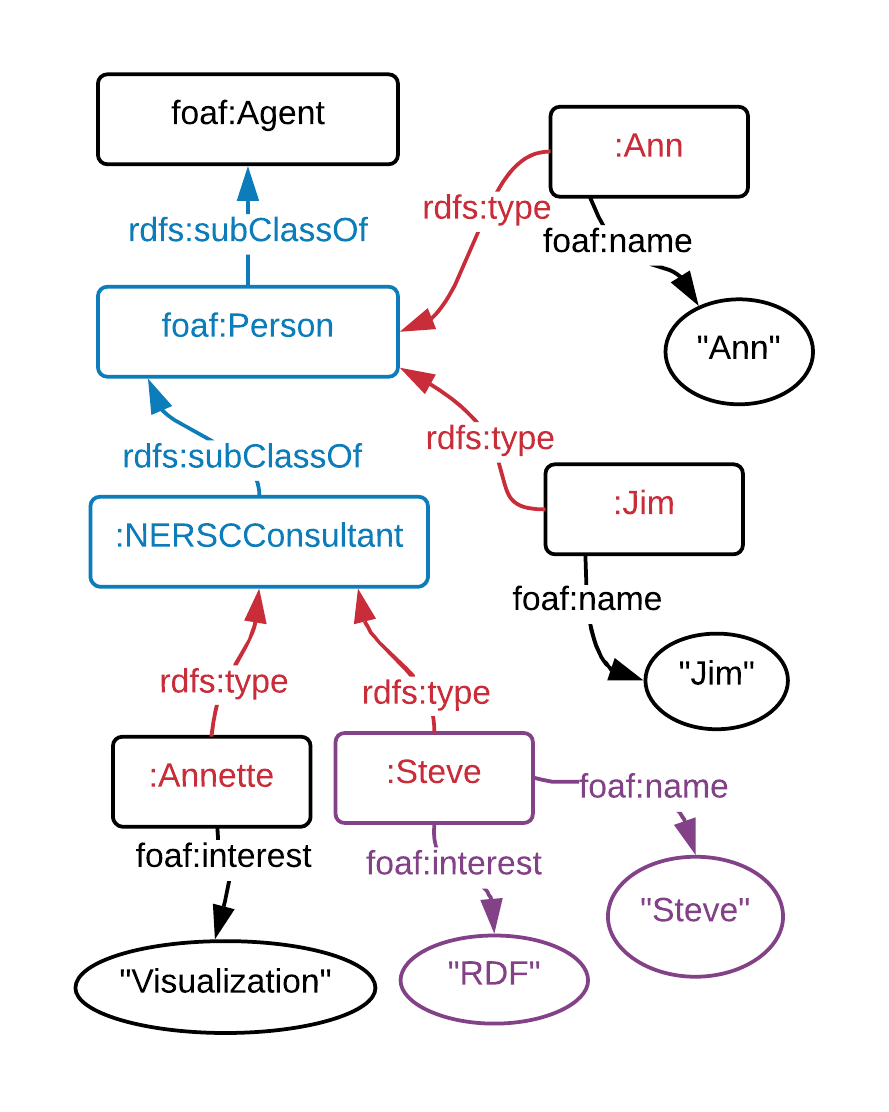
\includegraphics[width=0.4\textwidth]{sparql.png}
\caption{Illustration of the SPARQL query in Figure~\ref{f:sparql} }
\label{f:sparql-diagram}
\end{figure}

\textcolor{red}{TODO: draw this as a diagram, probably explains it better}
\textcolor{red}{TODO: prob need a ref to an "intro to semantic web" resource}

RDF provides a decentralized mechanism for publishing information in a
machine-readable and searchable way, neatly meeting our requirements
(2) and (5). Furthermore, RDF allows us to use an established ecosystem of 
tools and libraries to achieve our goals.

\subsubsection{The vocabulary}

The key classes and predicates forming our vocabulary are illustrated in 
Figure~\ref{f:logset-classes}. Figure~\ref{f:logset-classes-nodes} provides 
examples of nodes in a graph corresponding to each class, and an 
illustration of how RDF descriptions of different \texttt{LogSet}s published 
in different places form a single, global graph is show in 
Figure~\ref{f:logset-example}. Particularly, Figure~\ref{f:logset-example}
shows how the vocabulary can be used to publish data dictionaries 
describing different \texttt{SubjectType}s and \texttt{LogSeries}.

The vocabulary is extended and specialized 
from the Data Catalog Vocabulary \textcolor{red}{cite}. The meaning, 
reason and usage of each are as follows:

\begin{description}
\item[Catalog] \hfill

The \texttt{dcat:Catalog} class is used as an access point to LogSet datasets and 
to link disparate collections into a single graph. Catalogs are anticipated to be 
published at a site granularity: staff at a site would publish LogSets under
a URL that the staff member can access, linked to the global graph via a single 
entry in the site Catalog. (The mechanism for this can be as simple as a pull
request to a Github repository).

\texttt{Catalog}s can use \texttt{rdfs:seeAlso} properties to link to other 
catalogs and to data dictionary

\item[LogSet] \hfill

A collection of logs related in system and access and timespan,
for example the logs collected in a \texttt{p0-} directory in the SMW of a Cray
XC for a single boot session. The \texttt{LogSet} should provide a description
of the data and contact information and is an entry point to metadata for 
the \texttt{ConcreteLog}s.

Note that the \texttt{LogSet} itself doesn't necessarily have properties for 
temporal or subject information. We anticipate that these would be derived 
from the \texttt{ConcreteLog}s comprising the \texttt{LogSet}.

A \texttt{LogSet} might be a closed archive or might be ``open'', that is' 
acquiring new logs over time. This is indicated via the \texttt{isClosed} 
property, ..

\item[ConcreteLog] \hfill

A \texttt{ConcreteLog} describes a specific, concrete source of log entries.
This might be a log file but could also be, for example, a Slurm instance
from which job data can be obtained. 

The \texttt{accessURL} and \texttt{downloadURL} have subtly different uses,
inherited from \texttt{dcat:Distribution}. The actual data described by the 
\texttt{ConcreteLog} may not be directly accessible (due to security or 
other practical constraints), in which case an \texttt{accessURL} which 
can help a user to learn about gaining access is more suitable than a 
\texttt{downloadURL}, which is expected to provide direct access to the 
data.


The \texttt{ConcreteLog} also supports a number of properties about the
size, number of records and timespan of the data. For many data sources 
an ill-considered query might result in an excessive volume of data returned,
so these properties are intended to help users check 


\item[LogSeries] \hfill

The console log for a server is often distributed over multiple files,
and is fundamentally the same for servers of the same make at different
sites. A \texttt{LogSeries} allows the common metadata to be published
once in a common dictionary...


\item[LogFormatType]

One level more general than a \texttt{LogSeries}, a \texttt{LogFormatType}
is common to many \texttt{LogSeries}. As an example, many \texttt{LogSeries}
have the form of a \texttt{timeStampedLogFile}. Another significant 
\texttt{LogFormatType} is \texttt{sqlite3DB} (which encapsulates our 
reference implementation of the Annotation Schema~\textcolor{red}{cross-ref})

\item[Subject]
...
affects and partOf



\item[SubjectType]

Each \texttt{ConcreteLog} has a specific \texttt{Subject} - e.g. a 
\texttt{cori} or \texttt{cori\_nid00123}. It is useful to classify 
\texttt{Subject}s by their type so that for example, a researcher 
seeking HSN data can find \texttt{ConcreteLog}s about the HSN 
component of multiple clusters by querying for \texttt{ConcreteLogs}
whose \texttt{subject} is a specific \texttt{subjectType}. 

This also supports cataloging new datasets: rather than asking the
user the \texttt{subject} of each \texttt{ConcreteLog}, we can 

skos:broader, also aspectof


\end{description}

-- some key things to call out:
\begin{itemize}
\item someone publishing a logset doesn't need to know many people to get their 
      logset into the graph - a curator of their local (site) catalog is enough. 
      That curator then knows curators of at least one other catalog and thus 
      gets the local 
      subgraph into the global graph
\item someone using the graph doesn't need to know who published what - they can
      query the graph itself and get metadata about what is out there, including contact 
      information for data they don't directly have access to. This allows them to 
      solve specific access limitations in a locally-appropriate way
\end{itemize}

\begin{figure*}
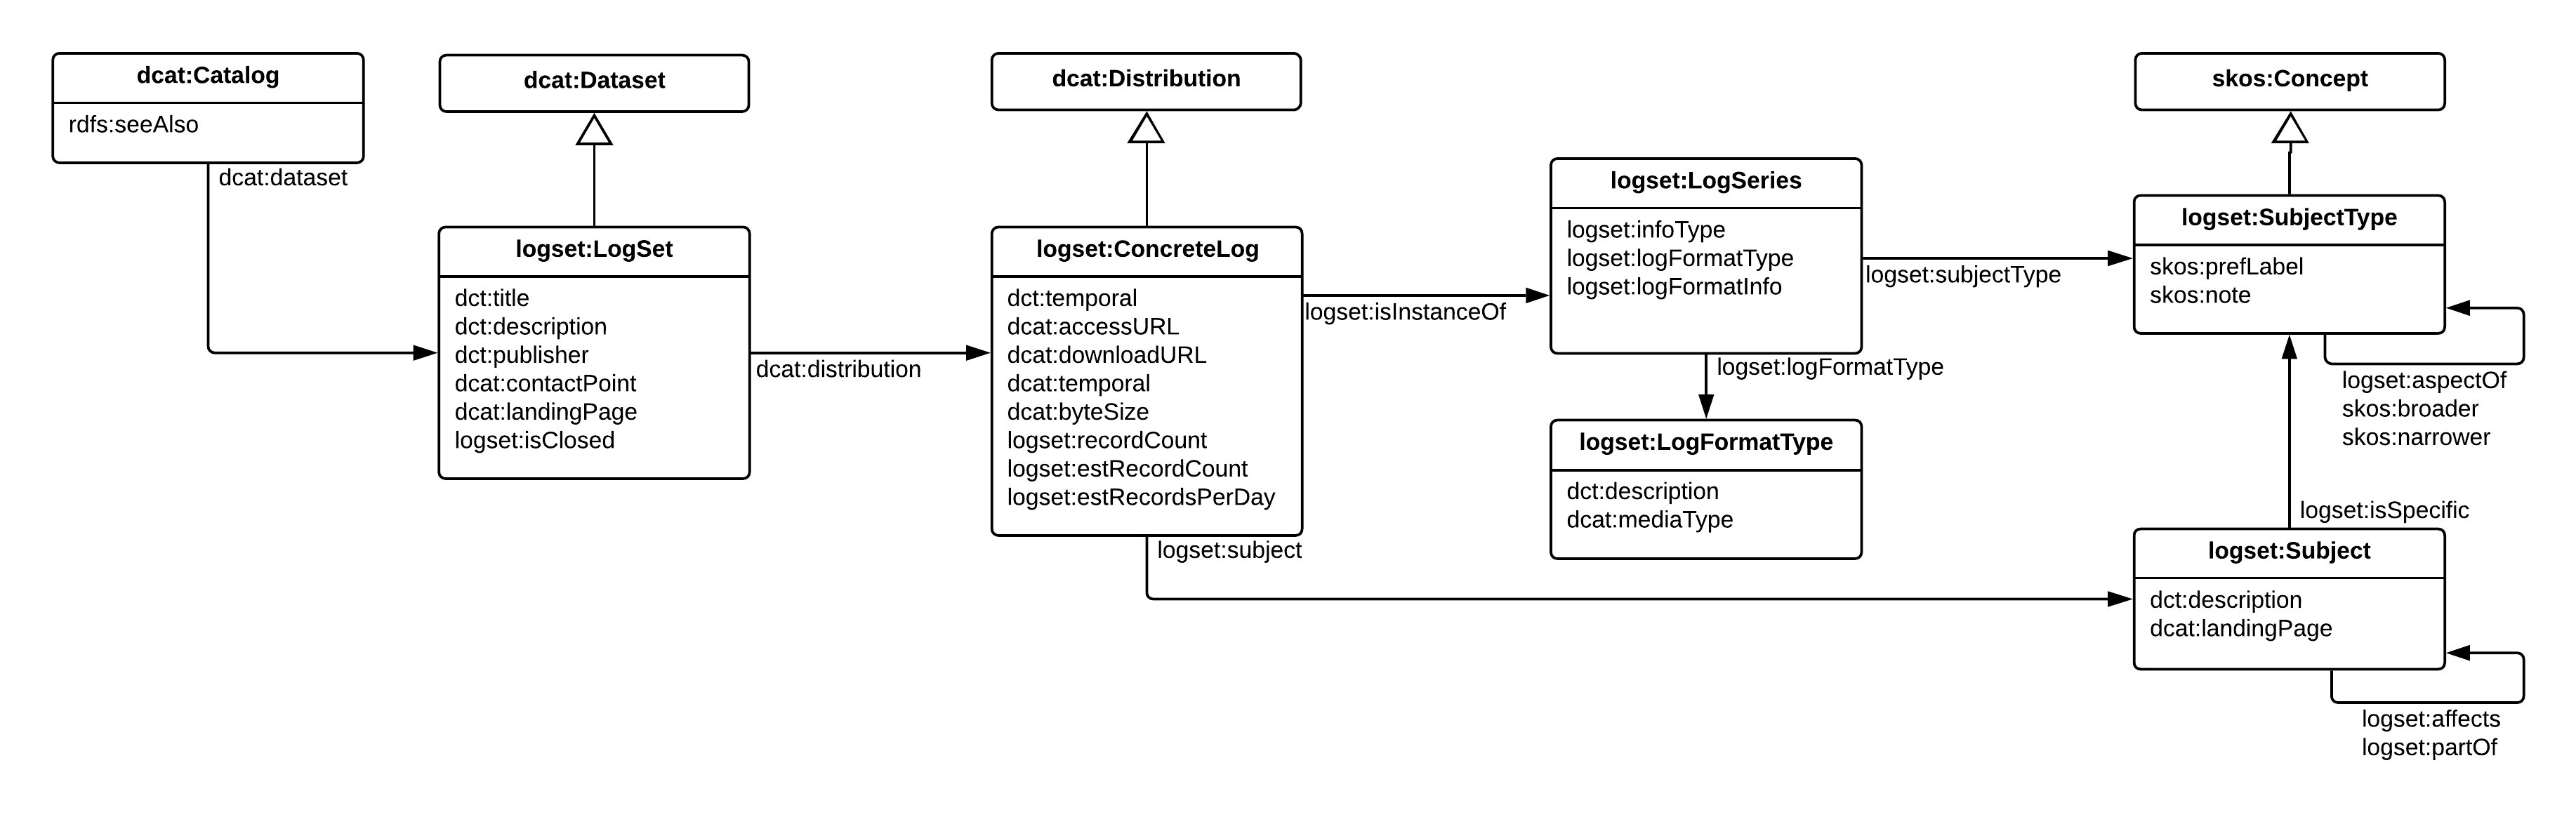
\includegraphics[width=1.0\textwidth]{logset-key-classes.png}
\caption{Key classes and predicates in the logset vocabulary. }
\label{f:logset-classes}
\end{figure*}

\begin{figure*}
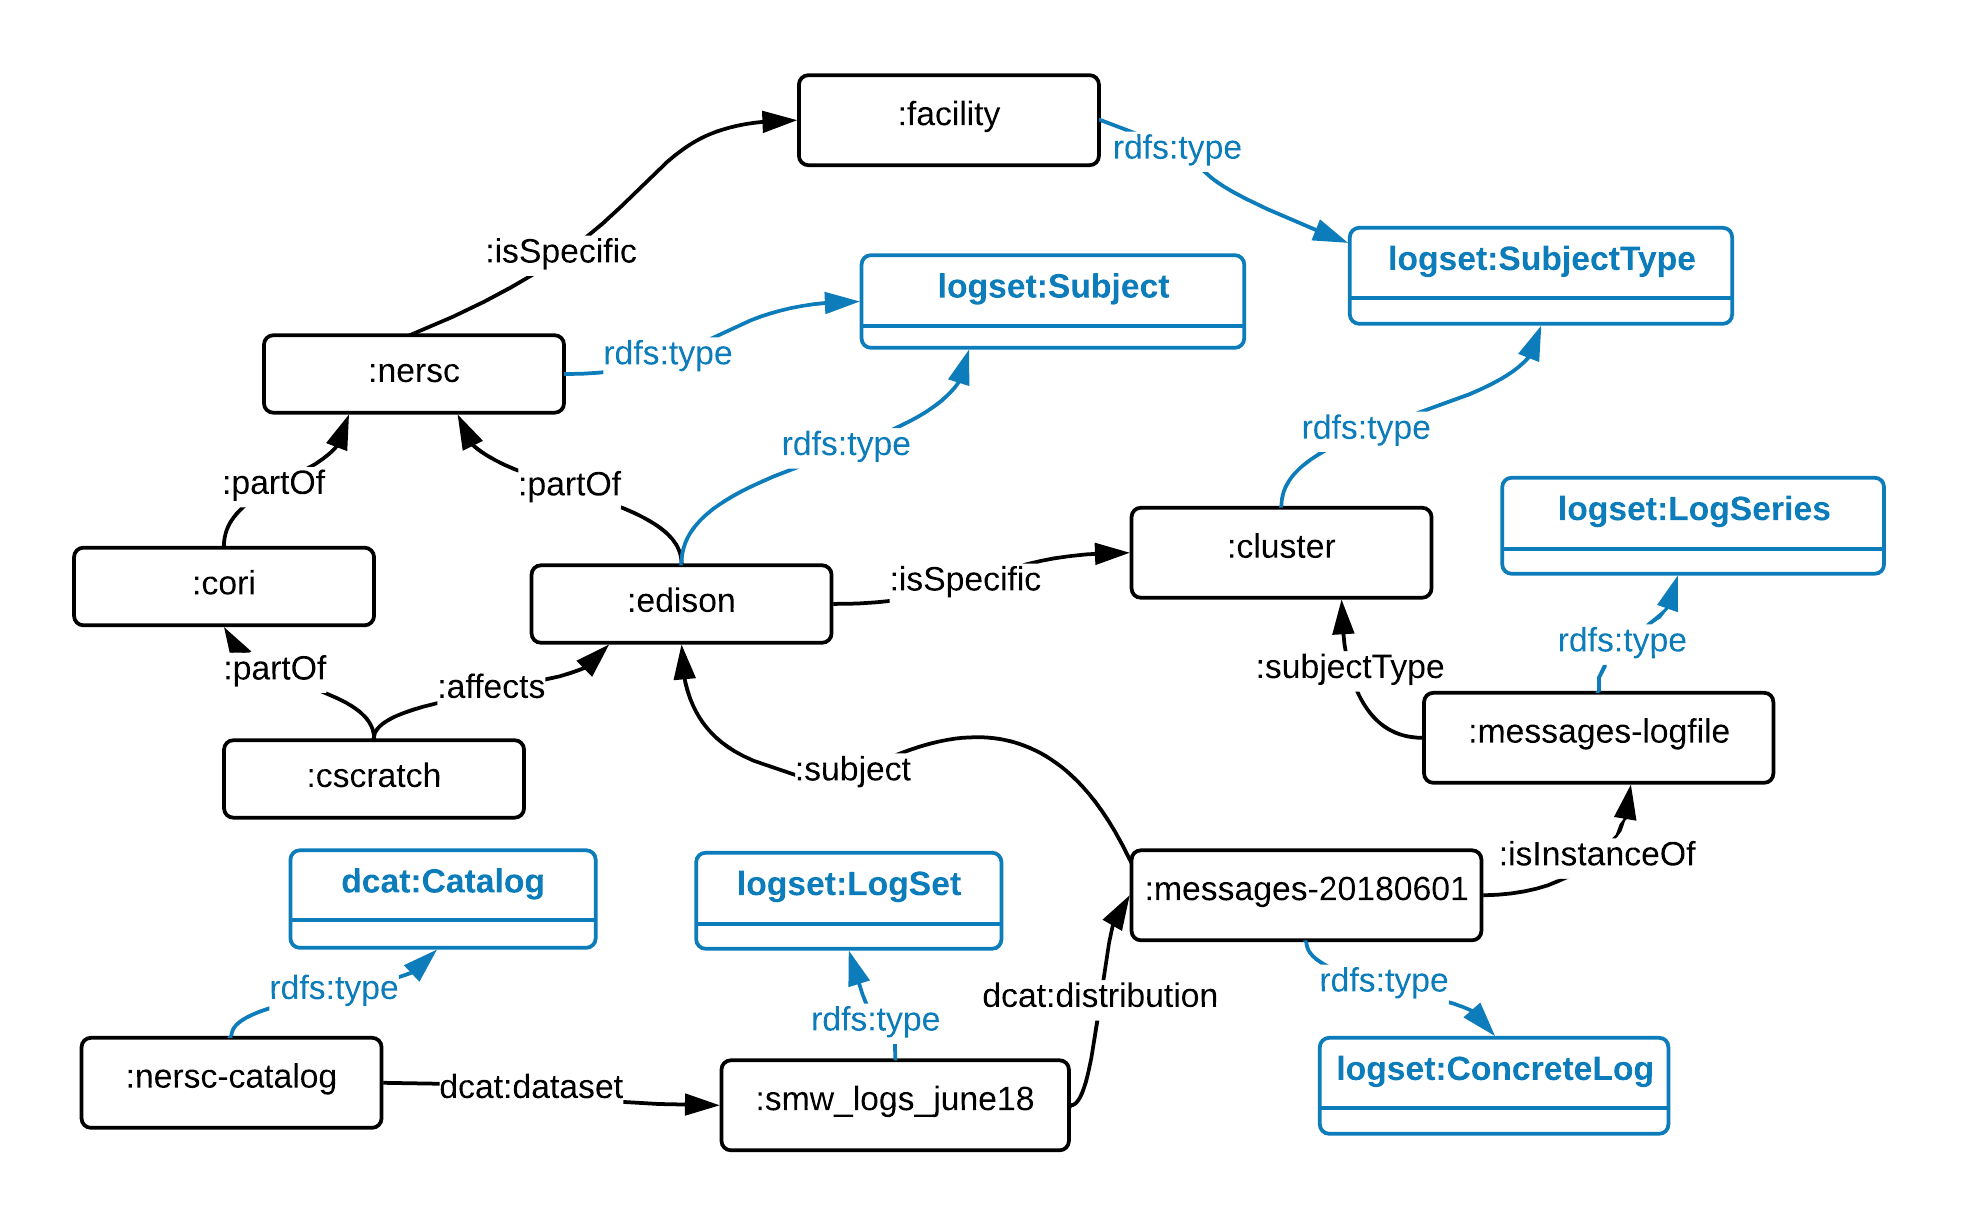
\includegraphics[width=0.9\textwidth]{logset-classes-nodes.png}
\caption{Examples of some nodes and relationships published in different places 
from different sites (indicated via color), forming a single global graph. }
\label{f:logset-classes-nodes}
\end{figure*}

\begin{figure*}
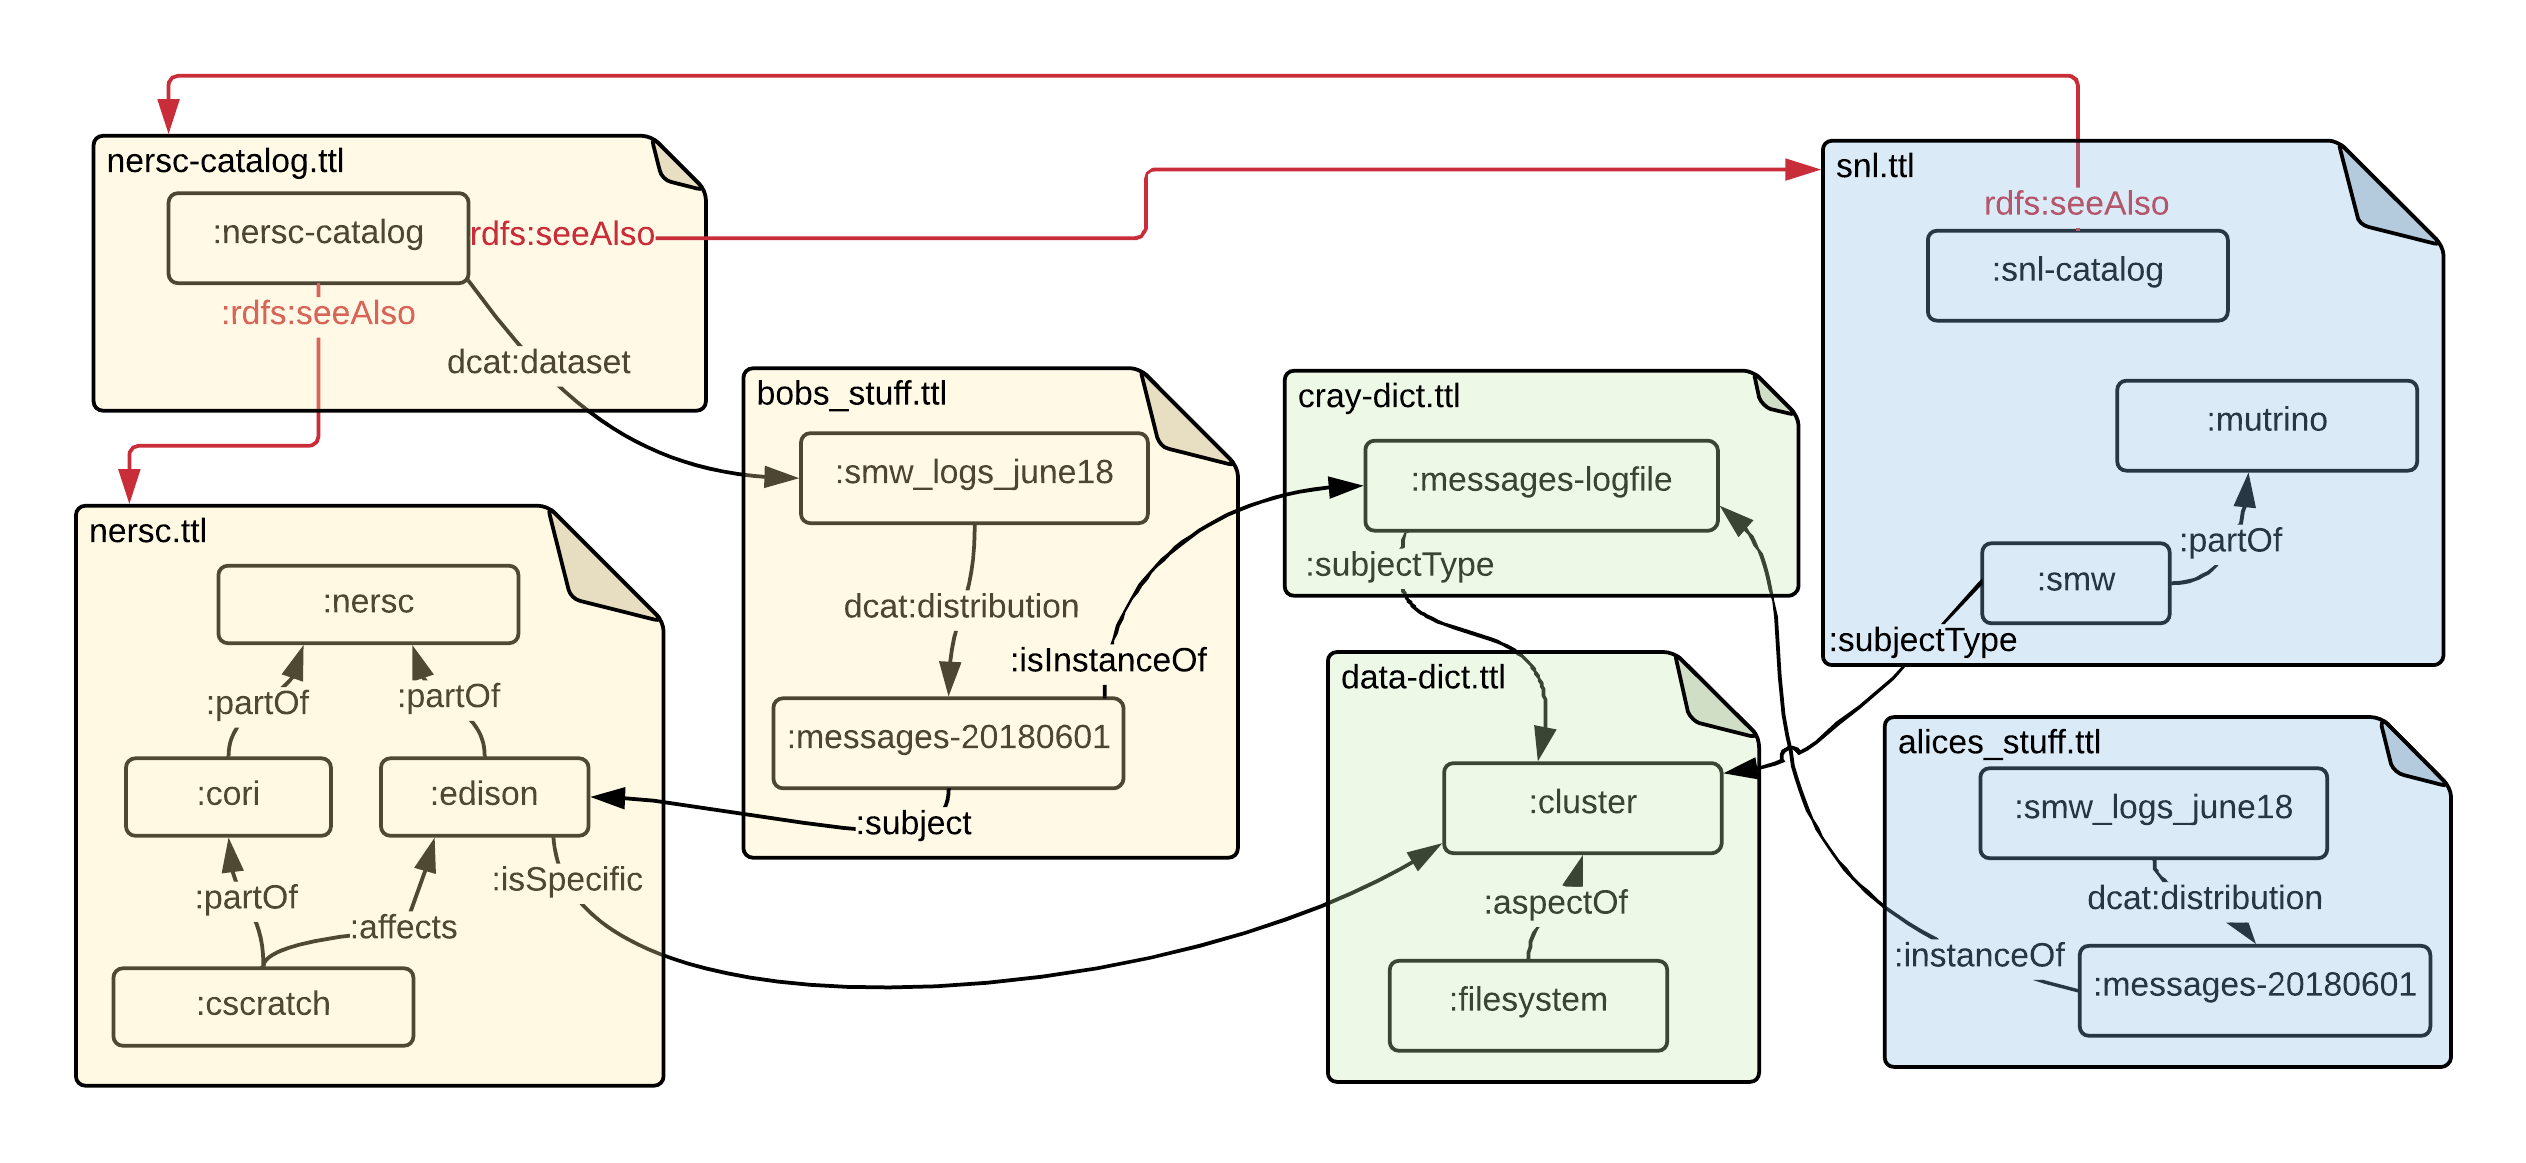
\includegraphics[width=0.9\textwidth]{logset-example.png}
\caption{Key classes and predicates in the logset vocabulary. }
\label{f:logset-example}
\end{figure*}

\subsection{Annotation Schema}

The primary goal of annotation is to provide a reduced
Some specific requirements influencing the design of our annotation schema
are:

\begin{itemize}
\item 
\item Temporal and subject (system and component) information are 
      the key fields, along with a human readable description, the 
      annotation itself.
\item The raw logfiles that the annotation concerns should be identified,
      if possible.
\item Multiple people should be able to annotate the same underlying 
      log data, and users of the annotations should be able to 
      identify annotators to request more information, if necessary.  
\item The architectural relationships between components indicated in 
      annotations should be accessible, in order to facilitate 
      traversal from an annotation of interest to annotations relating to
      components that may have impacted it.
\item Annotation fields should support searching based on the subject type 
      of an annotated event (such as a network event) or other 
      related information.
\end{itemize}



\begin{figure}
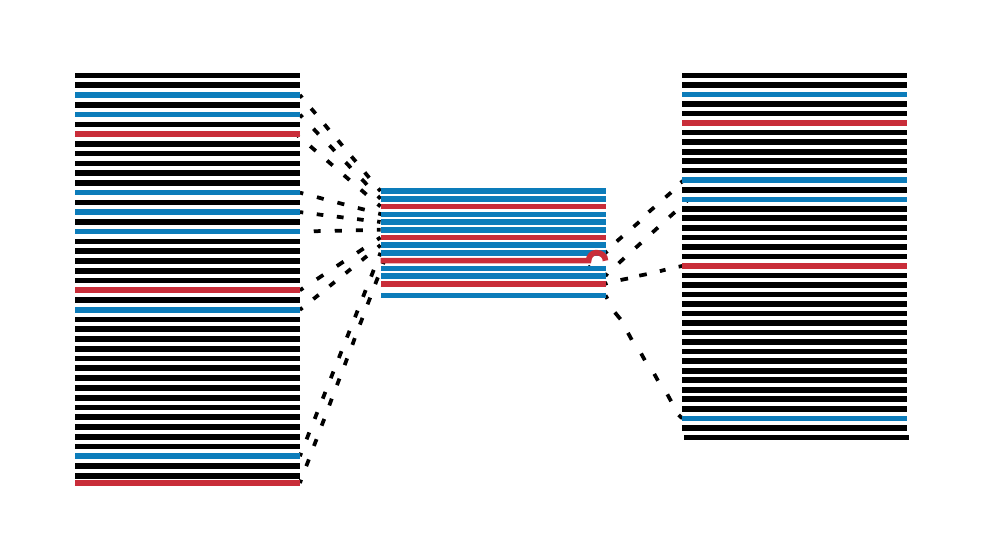
\includegraphics[width=0.4\textwidth]{annotations.png}
\caption{Annotations can collate a tractable subset of data from multiple log files into a single location.  }
\label{f:annotations}
\end{figure}

\begin{description}
\item[Catalog] \hfill

\end{description}

%In this subsection we describe the major fields necessary to support the
%architectural requirements that pertain to the annotations themselves
%(as opposed to the remote discovery infrastructure). The prototype
%implementation is an SQLite database, so we descirbe in in terms
%of that implemention, however that is not required. More generally
%this would be descirbed in terms of accessor APIs independent of
%the implementation beneath them.
The annotation schema is an SQL database definition with a central ``annotations'' table. Significant fields in the annotations table are:

The annotations table is defined as:
\begin{small}
\begin{minted}{sql}
CREATE TABLE 'annotations' (
       id             integer,
       authorid       char(3) NOT NULL,
       description    text NOT NULL,
       -- timespan of the action or event:
       starttime      datetime NOT NULL,
       endtime        datetime NOT NULL,
       -- impact of the action or event:
       startstate     text,
       endstate       text,
       systemdown     boolean,
       system         text,
       components     text,
       -- was the event manually induced?
       manual         boolean,
       -- subject type and annotation context:
       LDcatgroup     text, REFERENCES 'LDgroups'
       LDcategory     text,
       LDtag          text,
       balerpatternid integer,
       -- event source:
       logfiles       text,
       PRIMARY KEY('id','authorid')
        );
\end{minted}
\end{small}

The major fields for an annotations include \texttt{description}, \texttt{starttime}, \texttt{end time},
\texttt{system}, and \texttt{components} involved.
The description is a descriptive translation of a log messge or event (Examples
are given in Section~\ref{s:examples}); it is this description to which we
mainly refer when we refer to an annotation.
The \texttt{authorid} identifies the author of an annotation, who
is responsible for the determination of the content of the assignable fields
(such as the description); the authorid and annotation id together form a unique key.
Time and component fields refer to a specific instance of a log line or event
occurence. Thus multiple annotated log line instances may share the same description,
but have different time and component values.

Other information is used to help with context and search.
For example, \texttt{startstate} and \texttt{endstate}, which
are subjective and can be used to record things like a component
that starts a faulty but is repaired by the action of the annotations,
for example, if the event is recording that a DIMM was changed.
\texttt{Systemdown} is meant to aid in the search for events that result
in full system failure.

\texttt{Manual} is used to indicate manually performed
events, such as an administrator action to take down a node as opposed
to the system taking down a node because it failed a health check.
Knowledge of this can be used to more accurately determine the
number of true failure events and for assessing the effectiveness
and availability of system resilience mechansims vs required
human intervention.

A set of fields, \texttt{LDXXX} are available to give contextual inforatmion.
At the moment only \texttt{LDcategory} is used; this is used to define the major
subsystem relevant to the annotation. The current options are: \texttt{node/blade},
\texttt{scheduler}, \texttt{storage}, \texttt{network}, \texttt{cooling/facilities/sensors},
\texttt{power}, \texttt{system software}, \texttt{datawarp}, and \texttt{unknown}.

Note that event may have many relationships. We choose to limit them to one each to address
the requirement of searchability. It is expected that exploration will facilitate dsicovery
of events, even when the first order assocation may be off; also discovery of assocationed
events in different subsytems can help understanding of how events propagate in a system.

Annotations may also refer to other annotations; this is called a \texttt{metaannotation}.
An example might be where an annotation refers to a particular facilities
test and a meta annotations refers to the entire set of tests.

\texttt{Components} can include the compute and any supporting subsystems,
such as storage and facilities related elements. For the Cray system
itself, we define \texttt{node}, \texttt{blade}, \texttt{chassis},
\texttt{cabinet}, \texttt{router}, \texttt{tile}, \texttt{link}, \texttt{nic},
\texttt{smw}, and \texttt{other}.

In order to enable dsicovery of events which are either reported on related
compoentns or that propagate amont components we support the defintion
of \texttt{architectures}. For the Cray system itself, we define three.

The \texttt{physical} architecture consists of parent-child or
container-contained assocations, such as a cabinet is the parent of
3 chassis. For the network components, the router is a child of the blade.
he router is a parent of the links and nics. The physical architecture
can be populated from system defintation (e.g., XE or XC with the
correct number of cabinets for a system).

In order to support the fact that components may be identified by differnet
names in different log messages, an \texttt{alias} table defines those conventions.
This is largely cname, nid, and IP addresses determined from \texttt{/etc/hosts}
or the output for \texttt{rtr --system-map}.

The \texttt{router} architecture includes the network topology information
for the router (e.g., blue:black:green)
for Aries and X:Y:Z for gemini). The router information can be populated from
the system-map output or the otuput of \texttt{rtr --interconnect}.
The \texttt{link} architecture represents the network link connectivity,
consisting of type (e.g., Blue, X+) and the tile endpoints obtained
from the interconnect output.

The \texttt{link} architecuture supports determination if an event affects the
components at teh other end of a network link. The router architecutre
supports determination of proximity of events in the network topology.
We chose to separate architecutres in order to enable different
search and interpreation of events which affect components with
different \texttt{association} with each other. \texttt{associations}
include \texttt{parent-child: component-component} as opposed to
\texttt{parent-child: router tile}, or \texttt{peer: HSN link}
as opposed to \texttt{peer: Router-NIC} or \texttt{peer: NIC-Proc}.
To represent more globally associated, such as SMW
events which can directly affect all components, we define
a \texttt{supremum} relationship.

In the prototype, we define all architectures and relationships,
however we currently prinipally search the physical topology only
and support recursive search up and down, including for supremum
relationships. We are working on tools to better enable search of
the multiple architecture represenations.

In order to determine the effect of events on jobs, we also
intend that job data be made availble with the annotations.
We expect only the current common fields (e.g., starttime,
endtime, components, etc) exposed in scheulder logs or
interfaces.








\subsection{Tools}
\begin{itemize}
\item get.py for querying an annotation database
\item what do we have for building an annotation database? (Ann's tool for ingesting the mutrino and jobs info?)
\item framework for working with rdf graph

(plan is to have cataloging and running general queries supported at least, and ideally also slicing-and-fetching of timestamped logs in line-per-timestamp format)
\end{itemize}


- talk about why, eg rdf because it is machine readable, supports adding tools etc over time 


To faciliate the creation of log line annotaitons
and the identification of the occurences of events to be annotated,
we have been using two tools.

LogDiver~\cite{LogDiver} is a tool developed by UIUC which includes a set of regular expressions defining
events in log files of interest; the regular expressions are associated with categorizations
which are a subset of those described in the previous section; the
category name, \texttt{LDxxx}, was chosen to refelct our intention to map to the
Log Diver categroizations where possible.
LogDiver itself is used to discover the occurences of the regular
expresssions in the logs and to determine statistics and infroamtin about event sequences
such as statistics of failure events, or of timigns of failures and recoveries.
LogDiver, or any such regex-based tool (e.g., SEC~\cite{SEC}) can be used to efficiently extract events
and annotate them, based on the intention of the extistence of the regex.

For the dataset descirbed in this work, we prinicpally used Baler~\cite{Baler} for
identifying the log lines to be annotated and for extracing them from the dataset.
Baler extracts patterns from log files without requiring aprior knowledge of
regex. Rather, Baler takes dictionaries of ''words''; words appearing in the log lines
are the passed through to the pattern and non-words become a wildcard in the pattern.
Wildcards of certain formats, for example numbers, hex dumps, char arrays, hostnames and link names
(in cname format for Cray systems) are represented as that formatted type in the pattern.
For example, every instance of the log message \texttt{mutrino-smw 24626 found\_critical\_aries\_error: Processing ''PCI-e CMPL\_TIMEOUT'' critical error (0x660e)}
is represented by the pattern \texttt{<host> nlrd <pid> found\_critical\_aries\_error: Processing ''* *\_TIMEOUT'' critical error (<num>)}.
This illustrates where words, formatted wildcards, and unformatted wildcards (represented by \texttt{*}) appear in the pattern.

For Cray systems, we augment
the dictionary with an architecture specific dictionary of about 100 words (e.g., Lustre, DIMM).
For 3 months of data from our Trinity test system, Mutrino, a 100 node XC 40,
we had over 120 million text log lines which were reduced to 15500 patterns. To further identify patterns
of interest, we weight the patterns by the occurence of 50 weighted
keywords (e.g., congestion = 1.5, error = 1.5, degrade = 0.75). This further reduced the patterns
to 2500 significantly weighted patterns. For example the pattern
\texttt{<host> nlrd <pid> ***ERROR***: Link recovery operation failed; error <num>} has
an aggregate weight of 5.5. From those, we chose 150
patterns to annotate with enhanced descirptions. This resulted in about 860,000
annotated log line instances.

It is our intention to
build a plugin to interface with Baler, and support the annotations there,
however in the prototype, we merely annotated the extracted patterns from
Baler and loaded them into the database.
We do, however, include the Baler pattern id in the annotation fields
for reference ease; only the annotation description, not the original log line nor the pattern
are stored in the annotation database.

Some example patterns, from which the originating log line will be obvious, and
the resulting annotation used in this work, are given in Figure~\ref{f:baler}

\begin{figure*}
\begin{annol}

Baler pattern, preceeded by weight (W=#) and balerpatternid number:
(W=5)        258   HWERR[<host>][<num>]:<num>:SSID RSP A_STATUS_ORB_TIMEOUT Error:*=<num>:*=<num>:*=<num>
Annotation:
authorid:acg  description: 'ORB timeout waiting on outstanding request(s) in the buffer'  LDcatgroup: NE

Baler pattern and weight:
(W=3.75)     498   <host> nlrd <pid> do_set_alerts: <num> links failed, <num> blades failed, <num> blade critical faults, *_in_progress <num>, *_*_reroute <num>; reroute required
Annotation:
authorid:acg  description: 'Setting alerts due to failures. A network reroute is required' LDcatgroup: NE

Baler pattern and weight:
(W=3.25)     748   <host> nlrd <pid> ***ERROR***: Warm swap operation failed; error <num>
Annotation:
authorid:acg description: 'Warm swap failed. This is in response to a operation intended to reset/reinit/replace a component (including network components).' LDcatgroup: NO

Baler pattern and weight:
(W=1.5)      705   <host> nlrd <pid> responder_work_*: Top <num> nodes involved with network congestion
Annotation:
authorid:acg description 'System computing and listing congestion candidate applications' LDcatgroup:NE
\end{annol}
\caption{Example Baler patterns extracted from log lines and their annotated versions. Events to annotate are based on
knowledge of significant events. Annotation descriptions can provide additional context to non-self-explanatory log messages.}
\label{f:baler}
\end{figure*}

\begin{figure*}
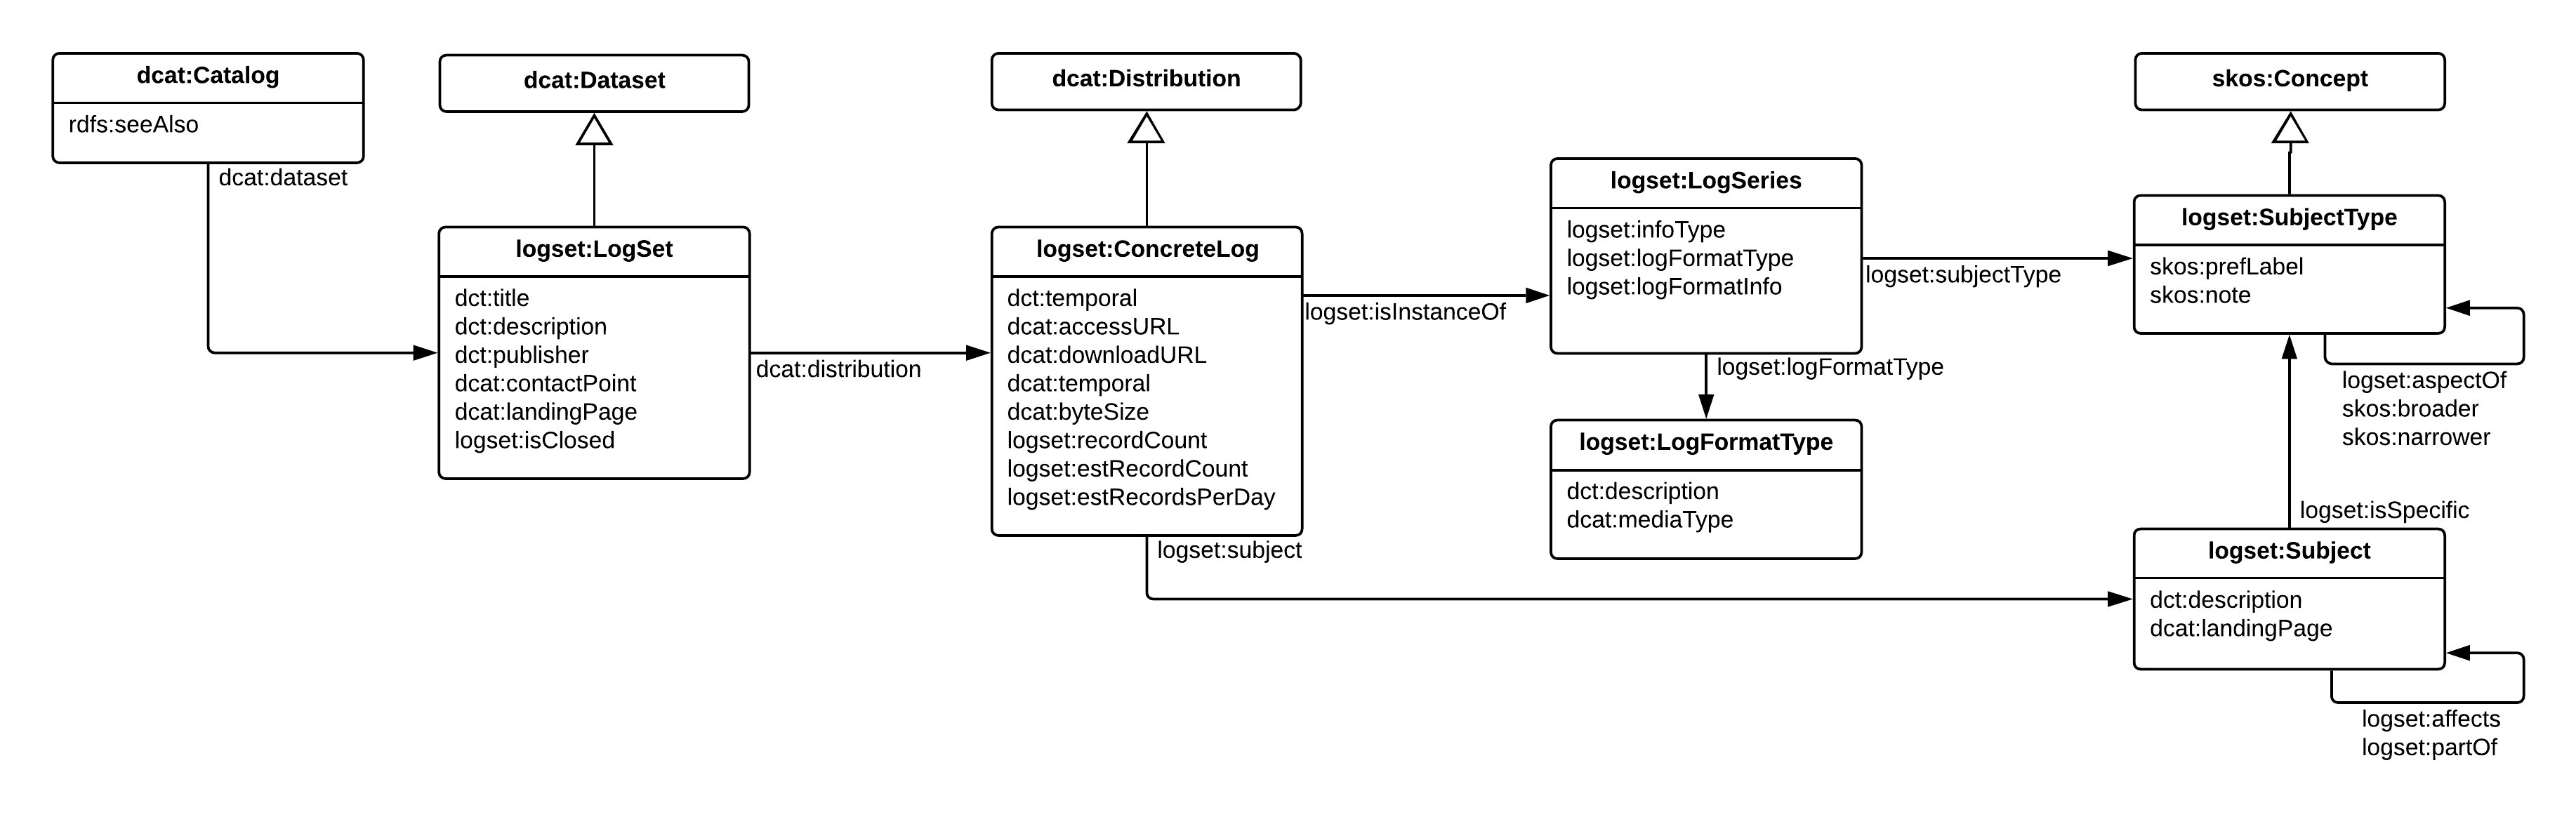
\includegraphics[width=0.9\textwidth]{logset-key-classes.png}
\caption{logset key classes}
\end{figure*}














\section{Case Studies}
\label{s:examples}
%%%%%%%%%%%%%%%%%%%%%%%%%

We show use of the annotations using the prototype implementation and tools. Examples
demonstrate the utility of the annotations in understanding
event occurrences and in problem diagnosis. They demonstrate that
the search space is greatly reduced from the whole log files, yet
the key events are revealed. They show how the annotations can be
used to drive further analysis in the log files. They show that
the descriptions can provide contextual information needed
for understanding events, thus lowering the barrier of
expert knowledge needed for understanding log events.

In these examples, we have presented our annotations in their current
state -- including typos and uncertainties in the interpretations.
We expect that this will be reflective of the annotations
in operation, with annotations evolving as additional authors
weigh in and additional expertise is obtained.

Note that some columns in the figures of annotation queries have been suppressed due to space
constraints. We explicitly retain the \texttt{balerpatternid} in the columns as this makes it easier
for the reader to associate individual instances of annotations of the same underlying event type
(e.g., same log message expect for a different component at a different time).
Colors in figures containing annotations are used to help call out annotations
referred to in the text.

\subsection{Job Impact}
\label{s:jobimpact}
%%%%%%%%%%%%%%%%%%%%%%%%%

We have annotated messages relating to potentially performance impacting conditions, including
thermal throttling events, power budgets exceeded, and memory errors. Example annotation
descriptions  include:
\begin{itemize}
\item \scriptsize\texttt{Correctable memory error.  This may result in degraded performance}\normalsize
\item \scriptsize\texttt{Blade or Cabinet controller taking correctable memory errors. This may affect performance.}\normalsize
\item \scriptsize\texttt{Package temperature above threshold (too hot). The CPU clock has been throttled. Should result in all threads for all cores will be throttled. This may affect application performance.}\normalsize
\end{itemize}

Of particular interest in XC systems is the ability to power cap. In such cases, not only is it of interest when
the power budget is exceeded, but also when caps are applied, or perhaps fail to be applied. Our annotation
system enables such events to be exposed to the user.
Many of these messages are identified by commands in the \texttt{commands} file or in the \texttt{controller} logs
and therefore are not typically released to users.
\RED{does the user get warned if setting the power cap fails to be applied?}

Examples include commands annotated as:
\begin{itemize}
\item \scriptsize\texttt{applying a power profile}\normalsize
\item \scriptsize\texttt{enforcing a power limit}\normalsize
\end{itemize}
error messages annotated as:
\begin{itemize}
\item \scriptsize\texttt{Error getting initial node power status. This may affect power capping.}\normalsize
\item \scriptsize\texttt{Error disabling power monitor. This may affect power capping.}\normalsize
\item \scriptsize\texttt{Node Error setting power budget. This may affect power capping.}\normalsize
\end{itemize}

A fundamental goal of the annotations is to enable user to understanding why performance and power limits did not perform as expected.
Basic capabilities enabled by our infrastructure include the ability to determine annotations occurring during a given job
and jobs running while an annotation occurred. Examples of each are given in Figure~\ref{f:powerbudget}.
In the top of the figure, all annotations during a job are queried -- it is seen that multiple times on multiple nodes, the
power budget is exceeded, which may result in performance impact. In the bottom of the figure jobs running while an annotation occurs are queried. In this case,
while the annotation was specific to node \texttt{c0-0c1s3n2}, the job itself was running on 96 nodes. Facilitating
tracing the propagation of impact of an event is one of the design goals of this work.

\begin{figure*}
\begin{annol}

# query for annotations during JobId 163510
python get.py -j 163510  -f table annotations
id	authorid	starttime	endtime		description	logfiles	LDcategory	components	balerpatternid
<@\textbf{\textcolor{red}{855158	acg	2015-05-03 01:12:16	2015-05-03 01:12:16	Node power budget exceeded.	controllermessages	PW	["c0-0c1s3n2"]	2871}}@>
<@\textbf{\textcolor{red}{864565	acg	2015-05-03 01:12:21	2015-05-03 01:12:21	Node now within power budget after it was exceeded.	controllermessages	PW	["c0-0c1s3n2"]	2872}}@>
<@\textbf{\textcolor{red}{855159	acg	2015-05-03 01:12:22	2015-05-03 01:12:22	Node power budget exceeded.	controllermessages	PW	["c0-0c0s11n0"]	2871}}@>
<@\textbf{\textcolor{red}{855160	acg	2015-05-03 01:12:23	2015-05-03 01:12:23	Node power budget exceeded.	controllermessages	PW	["c0-0c1s3n1"]	2871}}@>
<@\textbf{\textcolor{red}{...Occurs multiple times for multiple nodes...}}@>


# query for jobs running during annotation 864574
python get.py --jobs 855158 -f table annotations
JobId    UID    JobName    NumNodes    Start    End
<@\textbf{\textcolor{red}{('163510', XXX, ``'xhpl''', 96, '2015-05-03 00:51:24', '2015-05-03 01:19:15')}}@>>

\end{annol}
\caption{Annotations provide access to power state information in otherwise unavailable logs. Basic implementation
capabilities include discovery of annotations during a job (top) and and jobs running while an annotation occurred (bottom).}
\label{f:powerbudget}
\end{figure*}



\subsection{HSN Congestion}
\label{s:congestion}
%%%%%%%%%%%%%%%%%%%%%%%%%

In order to investigate network conditions, we chose to search for annotations involving the
word ''congest''. Query results are given in Figure~\ref{f:congest}. This looks like the
expected output of response to a congestion conditions, though it was suprising
on a system of this size, with candidate nodes and applications
as computed by the system.

\begin{figure*}
\begin{annol}
python get.py  -t congest -f table annotations

id	authorid	starttime	endtime		description	logfiles	LDcategory	components	balerpatternid
756163	acg	2015-04-28 10:15:44	2015-04-28 10:15:44	System computing and listing congestion candidate applications		nlrd	NE	["unknown"]	704
756168	acg	2015-04-28 10:15:44	2015-04-28 10:15:44	System computing and listing congestion candidate nodes		nlrd	NE	["unknown"]	705
...
756167	acg	2015-04-28 10:32:06	2015-04-28 10:32:06	System computing and listing congestion candidate applications		nlrd	NE	["unknown"]	704
756172	acg	2015-04-28 10:32:06	2015-04-28 10:32:06	System computing and listing congestion candidate nodes		nlrd	NE	["unknown"]	705
\end{annol}
\caption{Congestion response annotations occur 5 times within 15 minutes. The annotation regarding
candidate applications drove investigation of the \texttt{nlrd} log file, but no applications
were listed.}
\label{f:congest}
\end{figure*}

The annotation served as a guide to looking at the \texttt{nlrd} log to determine possible
applications of interest. \RED{This type of investigation would be enabled by the
full remote logset machinery}. There were, however, \emph{no} applications listed.
As a result, we then queried for all annotations around this time window to find indication
of a non-application congestion cause.

A query for annotations between 10:00 and 10:32 on that day resulted in 300 annotations, however there are only 7 distinct ones.
The reduction in log lines to annotation instances makes investigation of time ranges tractable and eases discovery
of similar event instances. Other than the ones in Figure~\ref{f:congest}, the rest dealt with problems with a single component \texttt{c0-0c1s8a0n0} and system
response to congestion.
\begin{itemize}
\item  192 occurences for component \texttt{c0-0c1s8a0n0} of \scriptsize\texttt{Correctable memory error.  This may result in degraded performance.}\normalsize
\item  47 occurences for component \texttt{c0-0c1s8a0n0} of \scriptsize\texttt{Component failed.}\normalsize
\item \scriptsize\texttt{Telling all blades to throttle network bandwidth. This should result in decreased network injection.}\normalsize
\item \scriptsize\texttt{Telling all blades to unthrottle network bandwidth. This should enable increased network injection.}\normalsize
\item \scriptsize\texttt{Unthrottling the service blades only}\normalsize
\end{itemize}


While we cannot be sure from the annotations alone that failure in this component was the cause of the congestion, it
is clearly a strong suspect.

Querying for annotations for \texttt{c0-0c1s8a0n0} revealed that the component's problems of these 2 types
started on 2015-04-02 10:22:47 and ended on 2015-04-30 at 07:16:52.
Narrowing down the root cause of the problems is difficult, however, because of a number of deliberately induced failures
during facilities testing which occurred that day. While we have put in a manual annotation for \scriptsize\texttt{Facilities testing}\normalsize,
the distributed system which we envision would have enabled the Facilities staff to annotate in more detail the exact testing which occurred.
Currently the \scriptsize\texttt{Facilities testing}\normalsize annotation has to serve as a indicator to examine the logs in which
indications of induced fan and power failures occurred.

The resolution of the problem is discovered by using a depth search to query annotations of related components: here \texttt{-d 2}
includes two levels of parents (\texttt{c0-0c1s8a0} and \texttt{c0-0c1s8}) children (none), and any unknown/supremum components.
The depth was chosen with the expectation that resolution would occur due to actions at the Aries or blade level.

While roughly 500 annotations occurred in response to the query,
only about 30 distinct annotations occurred. The annotations make it easy to understand the sequence of events. Extracted annotations are in Figure~\ref{f:congestresolve}.
First an annotation of a system administrator, 'abc', action, generically assigned to the day (green) confirms that the blade is being reseated in response
to errors. Warmswaps of the blade occur (cyan), however, while the warmswaps report as successful, timeouts waiting for items in the Outstanding Request Buffer (ORB)
result in the ORB being 'scrubbed', delaying the recovery (red). The annotations help with the understanding of the ORB scrub related events.
Eventually the blade is added back (green) successfully and the blade is then booted.

\begin{figure*}
\begin{annol}

python get.py  -c c0-0c1s8a0n0 -d 2 -s "2015-04-30 07:00:00" -e "2015-04-30 10:00:00" -f table annotations

id	authorid	starttime	endtime		endstate    description	logfiles	LDcategory	components	balerpatternid

<@\textbf{\textcolor{green}{4	abc	2015-04-30 00:00:01	2015-04-30 23:59:59	aries errors	blade reseated	Blade reseating in response to aries errors	NE	["c0-0c1s8"]}}@>
<@\textbf{\textcolor{cyan}{865013	acg	2015-04-30 07:10:14	2015-04-30 07:10:15	1	xtwarmswap remove	commands	NO	["c0-0c1s8"]}}@>
<@\textbf{\textcolor{cyan}{865797	acg	2015-04-30 07:15:50	2015-04-30 07:15:50	1	xtwarmswap remove	commands	NO	["c0-0c1s8"]}}@>
<@\textbf{\textcolor{cyan}{866043	acg	2015-04-30 07:16:47	2015-04-30 07:16:47	1	xtwarmswap remove	commands	NO	["c0-0c1s8"]}}@>
<@\textbf{\textcolor{cyan}{865976	acg	2015-04-30 07:16:55	2015-04-30 07:17:25	0	xtwarmswap remove	commands	NO	["unknown"]}}@>
766569	acg	2015-04-30 07:16:56	2015-04-30 07:16:56		Handling Warm swap for partition.	nlrd	NO	["unknown"]	455
866491	acg	2015-04-30 07:16:56	2015-04-30 07:16:56	0	xtcli set_alert		commands	NE	["c0-0c1s8a0"]
752251	acg	2015-04-30 07:17:03	2015-04-30 07:17:03		Setting alerts due to failures. A network reroute is required	nlrd	NE	["unknown"]	498
756229	acg	2015-04-30 07:17:10	2015-04-30 07:17:10		Quiescing the network. This should result in decreased network injection.	nlrd	NE	["unknown"]	509
756239	acg	2015-04-30 07:17:10	2015-04-30 07:17:10		Finished quiescing the network. (Is this just the steps in quiesce?).	nlrd	NE	["unknown"]	512
865961	acg	2015-04-30 07:17:16	2015-04-30 07:17:23	0	xtcli set_alert		commands	NO	["unknown"]
756132	acg	2015-04-30 07:17:25	2015-04-30 07:17:25		Telling all blades to unthrottle network bandwidth. This should enable increased network injection.	nlrd	NE	["unknown"]	423
756249	acg	2015-04-30 07:17:25	2015-04-30 07:17:25		Unquiescing the network. This will allow normal traffic injection to resume.	nlrd	NE	["unknown"]	554
756259	acg	2015-04-30 07:17:25	2015-04-30 07:17:25		Finished unquiescing the network. This will allow normal traffic injection to resume.	nlrd	NE	["unknown"]	557
<@\textbf{\textcolor{green}{766581	acg	2015-04-30 07:17:25	2015-04-30 07:17:25		Warm swap was successful. This is in response to a operation intended to reset/reinit/replace a component (including network components).	nlrd	NO	["unknown"]	566}}@>
766593	acg	2015-04-30 07:17:25	2015-04-30 07:17:25		The recovery operation for a failed link(s) was successful	nlrd	NE	["unknown"]	563
766603	acg	2015-04-30 07:17:25	2015-04-30 07:17:25		Done handling warm swap. This may not necessarily indicate success (?). This is in response to a operation intended to reset/reinit/replace a component (including network components).		nlrd	NO	["unknown"]	561
757133	acg	2015-04-30 07:17:42	2015-04-30 07:17:42		Starting to quiesce the node (node id might be in nodemask).		controllermessages	NE	["c0-0c1s8"]	2661
758693	acg	2015-04-30 07:17:42	2015-04-30 07:17:42		Finished quiescing the node.		controllermessages	NE	["c0-0c1s8"]	2666
<@\textbf{\textcolor{red}{763170	acg	2015-04-30 07:17:42	2015-04-30 07:17:42		Starting ORB scrub -- removing items in the Outstanding Request Buffer since its been too long for those messages	controllermessages	NE	["c0-0c1s8"]	2660}}@>
764343	acg	2015-04-30 07:17:52	2015-04-30 07:17:52		Finishing ORB scrub -- done removing items in the Outstanding Request Buffer since its been too long for those messages	controllermessages	NE	["c0-0c1s8"]	2669
760262	acg	2015-04-30 07:17:53	2015-04-30 07:17:53		Starting to unquiesce the node.		controllermessages	NE	["c0-0c1s8"]	2670
761831	acg	2015-04-30 07:17:53	2015-04-30 07:17:53		Finished unquiescing the node.		controllermessages	NE	["c0-0c1s8"]	2676
<@\textbf{\textcolor{red}{764926	acg	2015-04-30 07:17:53	2015-04-30 07:17:53		ORB timeout on node (nodes are in the message)		nlrd	NE	["unknown"]	435}}@>
<@\textbf{\textcolor{red}{757134	acg	2015-04-30 07:17:54	2015-04-30 07:17:54		Starting to quiesce the node (node id might be in nodemask).		controllermessages	NE	["c0-0c1s8"]	2661}}@>
758694	acg	2015-04-30 07:17:54	2015-04-30 07:17:54		Finished quiescing the node.		controllermessages	NE	["c0-0c1s8"]	2666
<@\textbf{\textcolor{red}{763171	acg	2015-04-30 07:17:54	2015-04-30 07:17:54		Starting ORB scrub -- removing items in the Outstanding Request Buffer since its been too long for those messages	controllermessages	NE	["c0-0c1s8"]	2660}}@>
764344	acg	2015-04-30 07:18:04	2015-04-30 07:18:04		Finishing ORB scrub -- done removing items in the Outstanding Request Buffer since its been too long for those messages	controllermessages	NE	["c0-0c1s8"]	2669
760263	acg	2015-04-30 07:18:05	2015-04-30 07:18:05		Starting to unquiesce the node.		controllermessages	NE	["c0-0c1s8"]	2670
761832	acg	2015-04-30 07:18:05	2015-04-30 07:18:05		Finished unquiescing the node.		controllermessages	NE	["c0-0c1s8"]	2676
<@\textbf{\textcolor{red}{764927	acg	2015-04-30 07:18:05	2015-04-30 07:18:05		ORB timeout on node (nodes are in the message)		nlrd	NE	["unknown"]	435}}@>

.....

<@\textbf{\textcolor{green}{866031	acg	2015-04-30 07:56:36	2015-04-30 08:03:27	0	xtwarmswap add	1	commands	NO	["c0-0c1s8"]}}@>
766571	acg	2015-04-30 07:56:39	2015-04-30 07:56:39		Handling Warm swap for partition.	nlrd	NO	["unknown"]	455
865720	acg	2015-04-30 07:56:39	2015-04-30 07:56:40	0	xtcli clr_alert	1	commands	NO	["c0-0c1s8"]
865819	acg	2015-04-30 07:56:39	2015-04-30 07:56:39	0	xtcli clr_alert	1	commands	NE	["c0-0c1s8a0"]
866784	acg	2015-04-30 07:56:40	2015-04-30 07:56:40	0	xtcli clr_warn	1	commands	NO	["c0-0c1s8"]
865012	acg	2015-04-30 07:56:46	2015-04-30 08:02:21	0	xtcli clr_warn	1	commands	NO	["c0-0c1s8"]
752253	acg	2015-04-30 08:02:22	2015-04-30 08:02:22		Setting alerts due to failures. A network reroute is required	nlrd	NE	["unknown"]	498
756231	acg	2015-04-30 08:03:08	2015-04-30 08:03:08		Quiescing the network. This should result in decreased network injection.	nlrd	NE	["unknown"]	509
756241	acg	2015-04-30 08:03:08	2015-04-30 08:03:08		Finished quiescing the network. (Is this just the steps in quiesce?).	nlrd	NE	["unknown"]	512
756251	acg	2015-04-30 08:03:23	2015-04-30 08:03:23		Unquiescing the network. This will allow normal traffic injection to resume.	nlrd	NE	["unknown"]	554
756261	acg	2015-04-30 08:03:23	2015-04-30 08:03:23		Finished unquiescing the network. This will allow normal traffic injection to resume.	nlrd	NE	["unknown"]	557
756134	acg	2015-04-30 08:03:24	2015-04-30 08:03:24		Telling all blades to unthrottle network bandwidth. This should enable increased network injection.	nlrd	NE	["unknown"]	423
<@\textbf{\textcolor{green}{766583	acg	2015-04-30 08:03:24	2015-04-30 08:03:24		Warm swap was successful. This is in response to a operation intended to reset/reinit/replace a component (including network components).	nlrd	NO	["unknown"]	566}}@>
766595	acg	2015-04-30 08:03:24	2015-04-30 08:03:24		The recovery operation for a failed link(s) was successful	nlrd	NE	["unknown"]	563
766605	acg	2015-04-30 08:03:24	2015-04-30 08:03:24		Done handling warm swap. This may not necessarily indicate success (?). This is in response to a operation intended to reset/reinit/replace a component (including network components).		nlrd	NO	["unknown"]	561
<@\textbf{\textcolor{green}{865000	acg	2015-04-30 08:08:34	2015-04-30 08:08:39	0	xtcli boot	1	commands	NO	["c0-0c1s8"]}}@>
\end{annol}
\caption{A blade reseating was performed to resolve blade problems which led to the congestion event.
Multiple iterations of scrubbing the Outstanding Request Buffer (ORB) were needed which
delayed resolution. The annotation of the system administrator (identified by 'abc') action supports the diagnosis.
}
\label{f:congestresolve}
\end{figure*}


The annotations additionally make it easy to compare and investigate timescales of similar events. For instance,
a recovery analysis might be based on the occurences and durtations of the warmswap sequences. This case
might appear of longer duration that others, and the interveniening ORB scrubbing events that
needed to be handled for full recovery would be easily apparent.


\subsection{Root Cause Diagnosis}
\label{s:route}
%%%%%%%%%%%%%%%%%%%%%%%%%
Another network investigation started with a search for annotations involving the word ''route''.
We were expecting to see events about reroutes triggered as a result of component failure. More interesting
are cases where the reroutes failed. Query output is shown in Figure~\ref{f:routeq}.

\begin{figure*}
\begin{annol}
# query for annotations where any text field contains the word 'route'
python get.py -t route -f table annotations

id	authorid	starttime	endtime	state	description	manual	logfiles LDcategory	components	balerpatternid
752245	acg	2015-02-27 11:53:08	2015-02-27 11:53:08	Setting alerts due to failures. A network reroute is required	nlrd	NE	["unknown"]	498
...
752255	acg	2015-05-08 07:54:15	2015-05-08 07:54:15	Setting alerts due to failures. A network reroute is required	nlrd	NE	["unknown"]	498
752256	acg	2015-05-08 08:11:47	2015-05-08 08:11:47	Setting alerts due to failures. A network reroute is required	nlrd	NE	["unknown"]	498
<@\textbf{\textcolor{red}{756223	acg	2015-05-08 08:17:46	2015-05-08 08:17:46	Error during computation of network route    nlrd	NE	["unknown"]	749}}@>
<@\textbf{\textcolor{red}{756224	acg	2015-05-08 08:31:24	2015-05-08 08:31:24	Error during computation of network route    nlrd	NE	["unknown"]	749}}@>
\end{annol}
\caption{Output of query for route annotations. Complete output = 15 annotations. Occurrences of network reroutes and failures in the rerouting process are of interest.}
\label{f:routeq}
\end{figure*}
%752254	acg	2015-05-08 07:35:42	2015-05-08 07:35:42	Setting alerts due to failures. A network reroute is required	nlrd	NE	["unknown"]	498

Each annotation \texttt{Setting alerts due to failures. A network reroute is required} makes clear that there has been a failure and what the next step in the response will be. It appears that 3 failures occurred that require network reroutes to recover and two of the computations of those route computations failed (red).

To understand why the route computation failed, we query for annotations during a time frame preceeding the event, limiting the options to network (NE) annotations only.
Query output is shown in Figure~\ref{f:routNEq}. There are only 24 total annotations as opposed to the raw log lines which total over 238,000.
It is clear from the annotations, that the component triggering the problem was \texttt{c0-0c0s9a0} and that
while the recovery operation for a failed link was successful (green), the
failure of the reroute was due to  a problem in adding the blade back to the HSN (to include it in the routing) (orange).


\begin{figure*}
\begin{annol}
# query for any annotations within the time range where the LDcategory is 'NE' (network)
python get.py -s ''2015-05-08 08:00:00'' -e ''2015-05-08 08:35:00'' -t LDcat=NE -f table annotations

id	authorid	starttime	endtime	description	manual	logfiles	LDcategory	components	balerpatternid
866450	acg	2015-05-08 08:11:42	2015-05-08 08:11:42	xtcli set_alert	1	commands	NE	["c0-0c0s9a0"]
752256	acg	2015-05-08 08:11:47	2015-05-08 08:11:47	Setting alerts due to failures. A network reroute is required	nlrd	NE	["unknown"]	498
756234	acg	2015-05-08 08:11:49	2015-05-08 08:11:49	Quiescing the network. This should result in decreased network injection.	nlrd	NE	["unknown"]	509
756244	acg	2015-05-08 08:11:50	2015-05-08 08:11:50	Finished quiescing the network. 		nlrd	NE	["unknown"]	512
756254	acg	2015-05-08 08:12:04	2015-05-08 08:12:04	Unquiescing the network. This will allow normal traffic injection to resume.	nlrd	NE	["unknown"]	554
756148	acg	2015-05-08 08:12:05	2015-05-08 08:12:05	Telling all blades to unthrottle network bandwidth. This should enable increased network injection.	nlrd	NE	["unknown"]	423
756264	acg	2015-05-08 08:12:05	2015-05-08 08:12:05	Finished unquiescing the network. This will allow normal traffic injection to resume.	nlrd	NE	["unknown"]	557
<@\textbf{\textcolor{green}{766598	acg	2015-05-08 08:12:05	2015-05-08 08:12:05	The recovery operation for a failed link(s) was successful	nlrd	NE	["unknown"]	563}}@>
864984	acg	2015-05-08 08:16:43	2015-05-08 08:16:43	xtcli clr_alert	1	commands	NE	["c0-0c0s9a0"]
<@\textbf{\textcolor{orange}{752223	acg	2015-05-08 08:17:46	2015-05-08 08:17:46	Marking HSN links down on blades that could not be added	nlrd	NE	["unknown"]	745}}@>
756149	acg	2015-05-08 08:17:46	2015-05-08 08:17:46	Telling all blades to unthrottle network bandwidth. This should enable increased network injection.	nlrd	NE	["unknown"]	423
<@\textbf{\textcolor{red}{756223	acg	2015-05-08 08:17:46	2015-05-08 08:17:46	Error during computation of network route	nlrd	NE	["unknown"]	749}}@>
866808	acg	2015-05-08 08:17:46	2015-05-08 08:17:46	xtcli set_alert	1	commands	NE	["c0-0c0s9a0"]
866328	acg	2015-05-08 08:30:21	2015-05-08 08:30:21	xtcli clr_alert	1	commands	NE	["c0-0c0s9a0"]
<@\textbf{\textcolor{orange}{752224	acg	2015-05-08 08:31:24	2015-05-08 08:31:24	Marking HSN links down on blades that could not be added	nlrd	NE	["unknown"]	745}}@>
756150	acg	2015-05-08 08:31:24	2015-05-08 08:31:24	Telling all blades to unthrottle network bandwidth. This should enable increased network injection.	nlrd	NE	["unknown"]	423
<@\textbf{\textcolor{red}{756224	acg	2015-05-08 08:31:24	2015-05-08 08:31:24	Error during computation of network route	nlrd	NE	["unknown"]	749}}@>
865971	acg	2015-05-08 08:31:24	2015-05-08 08:31:24	xtcli set_alert	1	commands	NE	["c0-0c0s9a0"]
\end{annol}
\caption{Output of query for network related annotations to investigate the cause of the failed routes. Complete output = 24 annotations.
A search of the raw log lines would be much more labor intensive -- 238,000 raw log lines occurred during this period.}
\label{f:routNEq}
\end{figure*}

This drives us to investigate problems with \texttt{c0-0c0s9}. Query output is shown in Figure~\ref{f:c0-0c0s9q}. The full output has 90 annotations, but there
are only a few distinct ones (shown). There is an out-of-memory killer annotation (red) that occurs repeatedly (repeats suppressed in the figure). Of particular interest is that the
out of memory problem is reported by the blade controller (file is controllermessages and component is the blade), as opposed to a user process being killed by
the OOM killer on a node.

While resolution of the exact cause of the problem may necessitate involvement of a vendor, it is at least obvious from this that the blade controller operating system believes it is experiencing a low memory condition and taking active measures to prevent complete failure. This could be due to a variety of reasons such as a memory leak, a communication problem causing buffering of messages to fill memory, etc. Unfortunately the processes it kills may be needed for proper operation and the problem being fixed by a complete reboot seems to validate that the problem was a software/firmware state issue and not hardware failure.

\begin{figure*}
\begin{annol}
# query for annotations within the time range and for the specified component
python get.py -s "2015-05-08 08:00:00" -e "2015-05-08 08:35:00" -c c0-0c0s9 -f table annotations

id	authorid	starttime	endtime	description	logfiles	LDcategory	components	balerpatternid
<@\textbf{\textcolor{red}{864619	acg	2015-05-08 08:06:48	2015-05-08 08:06:48	OOM kill process.		controllermessages	NO	["c0-0c0s9"]	2971}}@>
866418	acg	2015-05-08 08:11:40	2015-05-08 08:12:05	xtwarmswap remove	commands	NO	["c0-0c0s9"]
865065	acg	2015-05-08 08:13:00	2015-05-08 08:13:16	xtcli power down	commands	PW	["c0-0c0s9"]
865709	acg	2015-05-08 08:13:50	2015-05-08 08:15:12	xtcli power up	commands	PW	["c0-0c0s9"]
<@\textbf{\textcolor{red}{864620	acg	2015-05-08 08:13:51     2015-05-08 08:13:51	OOM kill process.		controllermessages	NO	["c0-0c0s9"]	2971}}@>
<@\textbf{\textcolor{red}{...REPEATS 6 Times}}@>
865955	acg	2015-05-08 08:16:41	2015-05-08 08:17:46	xtwarmswap add	commands	NO	["c0-0c0s9"]
864985	acg	2015-05-08 08:16:43	2015-05-08 08:16:43	xtcli clr_alert	commands	NO	["c0-0c0s9"]
865485	acg	2015-05-08 08:16:43	2015-05-08 08:16:43	xtcli clr_warn	commands	NO	["c0-0c0s9"]
865241	acg	2015-05-08 08:19:09	2015-05-08 08:19:09	xtwarmswap remove	commands	NO	["c0-0c0s9"]
865015	acg	2015-05-08 08:19:58	2015-05-08 08:19:58	xtcli halt	commands	NO	["c0-0c0s9"]
<@\textbf{\textcolor{red}{864624	acg	2015-05-08 08:21:01	2015-05-08 08:21:01	OOM kill process.	controllermessages	NO	["c0-0c0s9"]	2971}}@>
<@\textbf{\textcolor{red}{...REPEATS 5 Times}}@>
866482	acg	2015-05-08 08:21:21	2015-05-08 08:21:51	xtcli power down	commands	PW	["c0-0c0s9"]
865041	acg	2015-05-08 08:25:08	2015-05-08 08:26:29	xtcli power up	commands	PW	["c0-0c0s9"]
866012	acg	2015-05-08 08:30:18	2015-05-08 08:31:24	xtwarmswap add	commands	NO	["c0-0c0s9"]
865948	acg	2015-05-08 08:30:21	2015-05-08 08:30:21	xtcli clr_alert	commands	NO	["c0-0c0s9"]
866451	acg	2015-05-08 08:30:21	2015-05-08 08:30:21	xtcli clr_warn	commands	NO	["c0-0c0s9"]
\end{annol}
\caption{Output of query for annotations to investigate the cause of the component failure. Complete output = 90 annotations, about 10 of which are distinct. For example, the
node-related annotations occur for each node on the blade and many repeat in time and are suppressed in the figure. An OOM killer event occurs which is reported by the blade
controller, not a node.}
\label{f:c0-0c0s9q}
\end{figure*}


Finally, we are interested in determining if this problem got resolved and how. We utilize the depth search
\texttt{-d 1} to query parents (\texttt{c0-0c0}), children (the nodes and Aries), and any unknown/supremum components.
The depth and time range currently
are chosen by trial and error, however from output in Figure~\ref{f:routeresolution} it is clear that the OOM messages continue until an unsuccessful attempt is made to power
down the blade (orange), and a few attempts are necessary to reboot the system (red) and clear the alert (green). 

This case also illustrates
the endstate field (which is automatically populated with the end state of commands in the command file (described in Section~\ref{s:proof})). Note that erroneous commands, for example \texttt{xtcli power} with incorrect argument or target specified at 11:05:57, result in error. Also illustrated are manual attribution of any annotations of events from the \texttt{command} file and \texttt{p0-XXX} directories. The latter are
attributed to a generic system adminstrator authorid, \texttt{adm}, for the annotation, as opposed to the human annotation of the blade reseating in the previous example.

\begin{figure*}
\begin{annol}
# query for annotations between the time frame of interest for the named component and any components within a depth of 1
python get.py -s "2015-05-08 08:35:00" -e "2015-05-08 23:35:00" -c c0-0c0s9 -d 1 -f table annotations

id	authorid	starttime	endtime		endstate	description	manual	logfiles	LDcategory	components	balerpatternid
<@\textbf{\textcolor{orange}{865860	acg	2015-05-08 08:40:24	2015-05-08 08:40:54	0	xtcli power down	1	commands	PW	["c0-0c0s9"]}}@>
866403	acg	2015-05-08 08:51:18	2015-05-08 08:52:39	0	xtcli power up	1	commands	PW	["c0-0c0s9"]
865969	acg	2015-05-08 09:04:56	2015-05-08 09:05:09	0	xtcli power up	1	commands	PW	["c0-0c0s9"]
865426	acg	2015-05-08 10:55:04	2015-05-08 10:55:21	0	xtcli shutdown	1	commands	NO	["unknown"]
865427	acg	2015-05-08 10:59:07	2015-05-08 10:59:08	0	xtcli clr_alert	1	commands	NO	["c0-0c0s9"]
865429	acg	2015-05-08 10:59:07	2015-05-08 10:59:08	0	xtcli clr_alert	1	commands	NE	["c0-0c0s9a0"]
866614	acg	2015-05-08 10:59:08	2015-05-08 11:00:13	0	xtcli halt	1	commands	NO	["unknown"]
865078	acg	2015-05-08 11:00:29	2015-05-08 11:00:29	1	xtcli power on	1	commands	PW	["c0-0c0s9"]
866365	acg	2015-05-08 11:00:42	2015-05-08 11:00:53	0	xtcli power up	1	commands	PW	["c0-0c0s9"]
<@\textbf{\textcolor{orange}{766617	acg	2015-05-08 11:04:02	2015-05-08 11:04:02		Boot manager - halt request has failed		bm	NO	["unknown"]	15732}}@>
866399	acg	2015-05-08 11:04:02	2015-05-08 11:04:02	0	xtcli halt	1	commands	NO	["c0-0c0s9"]
865284	acg	2015-05-08 11:05:57	2015-05-08 11:05:57	1	xtcli power	1	commands	PW	["unknown"]
<@\textbf{\textcolor{red}{74	adm	2015-05-08 11:15:31		reboot (p0)	1			NO	["unknown"]}}@>
866035	acg	2015-05-08 11:15:42	2015-05-08 11:22:59	1	xtcli power up	1	commands	NO	["unknown"]
866268	acg	2015-05-08 11:26:54	2015-05-08 11:26:54	0	xtcli slot_off	1	commands	NO	["c0-0c0s9"]
864961	acg	2015-05-08 11:27:06	2015-05-08 11:27:06	1	xtcli power slot_off	1	commands	PW	["c0-0c0s9"]
866436	acg	2015-05-08 11:27:18	2015-05-08 11:27:48	0	xtcli power down_slot	1	commands	PW	["c0-0c0s9"]
<@\textbf{\textcolor{red}{75	adm	2015-05-08 11:55:20		reboot (p0)	1		NO	["unknown"]}}@>
866564	acg	2015-05-08 11:55:35	2015-05-08 11:57:04	1	xtcli power down_slot	1	commands	NO	["unknown"]
866547	acg	2015-05-08 12:42:12	2015-05-08 12:42:12	1	xtcli power slot_off	1	commands	PW	["c0-0c0s9"]
866460	acg	2015-05-08 12:42:21	2015-05-08 12:42:52	0	xtcli power down_slot	1	commands	PW	["c0-0c0s9"]
865783	acg	2015-05-08 12:43:11	2015-05-08 12:43:11	0	xtcli disable	1	commands	NO	["c0-0c0s9"]
<@\textbf{\textcolor{red}{76	adm	2015-05-08 12:43:43		reboot (p0)	1			NO	["unknown"]}}@>
864945	acg	2015-05-08 12:43:54	2015-05-08 12:50:15	0	xtcli disable	1	commands	NO	["unknown"]
<@\textbf{\textcolor{green}{866412	acg	2015-05-08 12:50:18	2015-05-08 12:50:18	0	xtcli clr\_alert	1	commands	NE	["c0-0c0s9a0"]}}@>
\end{annol}
\caption{Output of query for annotations to investigate the resolution of the component failure. Attempts to address the blade itself were unsuccessful,
and several reboots were required before the alert cleared.}
\label{f:routeresolution}
\end{figure*}





\section{Conclusions}
\label{s:conclusions}

% conference papers do not normally have an appendix


% trigger a \newpage just before the given reference
% number - used to balance the columns on the last page
% adjust value as needed - may need to be readjusted if
% the document is modified later
%\IEEEtriggeratref{8}
% The "triggered" command can be changed if desired:
%\IEEEtriggercmd{\enlargethispage{-5in}}

% references section

% can use a bibliography generated by BibTeX as a .bbl file
% BibTeX documentation can be easily obtained at:
% http://www.ctan.org/tex-archive/biblio/bibtex/contrib/doc/
% The IEEEtran BibTeX style support page is at:
% http://www.michaelshell.org/tex/ieeetran/bibtex/

%%%% YOU CAN ADD IN ADDITIONAL BIB FILES BELOW %%%

\bibliographystyle{IEEEtran}
%\bibliography{IEEEabrv,./test}
% argument is your BibTeX string definitions and bibliography database(s)
%\bibliography{IEEEabrv,../bib/paper}
\bibliography{IEEEabrv,./cug2018}
%
% <OR> manually copy in the resultant .bbl file
% set second argument of \begin to the number of references
% (used to reserve space for the reference number labels box)
%\begin{thebibliography}{1}
%\end{thebibliography}




% that's all folks
\end{document}
